%!TEX root = jt-thesis-main.tex

\section*{English Abstract}
\addcontentsline{toc}{section}{English Abstract}
\begin{onehalfspace}
    Gathering data from sensor networks entails challenges such as minimizing
    network latency, providing data accuracy, scaling the system, and, if the
    sensor nodes are battery powered, managing energy and sensor node lifetime.
    As the number of sensor nodes or data sources, increases so does the
    quantity of the produced data. Sampling algorithms are used to reduce the
    generated data at or near data sources and therefore to minimize network
    load. Sampling algorithms have advantages, limitations and some are use
    case specific. To provide an overview of existing sampling algorithms and
    the challenges of sensor data gathering we present a catalog of sampling
    algorithms for sensor data. We classify the presented sampling algorithms
    and order them into a taxonomy. We first divide sampling algorithms into
    sampling and filtering algorithms. We then further divide the sampling
    algorithms into adaptive sampling and compressive sampling. Likewise, we
    divide the filtering algorithms into model-based schemes and adaptive
    filtering algorithms. We provide a detailed overview of sampling algorithms
    and summarize their assumptions, advantages, limitations and message
    overhead. Additionally, we present and summarize algorithms from related
    areas, i.e., routing and topology control, algorithms which combine
    sampling techniques. We additionally highlight possible combinations of
    algorithms proposed by different authors.
\end{onehalfspace}
\clearpage

\section*{Deutscher Abstract}
\addcontentsline{toc}{section}{German Abstract}
\begin{onehalfspace}
    Das Sammeln von Daten aus Sensornetzwerken bringt Herausforderungen mit
    sich: Geringhaltung der Netzwerk Latenz, Zustellung genauer Daten,
    Skalierung des Netzwerkes und Energieverwaltung der Sensorknoten, wenn es
    sich um ein kabelloses Sensor Netzwerk handelt. Mit steigender Zahl von
    Sensorknoten, oder Datenquellen, steigt auch die Menge an produzierten
    Daten. Sampling Algorithmen werden verwendet, um produzierte Daten an oder
    in der Nähe von Datenquellen zu reduzieren und um somit die Belastung für
    das Netzwerk zu reduzieren. Sampling Algorithmen haben Vorteile,
    Einschränkungen und verschiedene Anwendungsgebiete. Um einen Überblick zu
    den existierenden Sampling Algorithmen und den Herausforderungen in dem
    Sammeln von Sensordaten bereitzustellen, stellen wir einen Katalog von
    Sampling Algorithmen für Sensor Daten vor. Wir klassifizieren die
    präsentierten Sampling Algorithmen nach Sampling und Filtering Algorithmen
    und Ordnen sie in einer Taxonomie. Wir unterteilen Sampling Algorithmen
    weiter in Adaptive Sampling und Compressive Sampling Algorithmen. Auch
    unterteilen wir die Filtering Algorithmen weiter in Model Based Schemes und
    Adaptive Filtering Algorithmen. Wir stellen einen Überblick von Sampling
    Algorithms dar und fassen deren Annahmen, Vorteile, Einschränkungen und
    Message Overhead in einer Tabelle zusammen. Zusätzlich präsentieren wir
    Algorithmen von verwandten Bereichen, nämlich Routing und Topology Control,
    und Algorithmen, welche Methoden von verschiedenen Klassen unserer
    Taxonomie verwenden. Wir zeigen zusätzlich mögliche Kombinationen von
    Algorithmen, die von verschiedenen Autoren vorgestellt wurden.
\end{onehalfspace}
\clearpage


\section{Introduction}
\label{sec:Introduction}
Gartner Inc. states that the number of network-connected devices will reach
20.4 billion by 2020~\cite{gartner}. To gather information from those devices,
we need algorithms which efficiently sample and route data from sensor nodes
(i.e., devices) to data sinks. Energy expenditure will gain higher importance,
especially for mobile devices such as battery-powered wearables and
smartphones. A \ac{WSN} is often battery-powered and use cases span from home
and health applications to the military sector~\cite{akyildiz2002wireless}.
With low production costs of a sensor node as a goal in
\acp{WSN}~\cite{akyildiz2002wireless}, resource usage at the sensor nodes is
restricted. While reducing sampling frequencies leads to a higher life of a
battery-powered sensor network, important changes in the observed phenomenon
could be missed which reduces the quality of the
data~\cite{akyildiz2002wireless}. A tradeoff between the quality of data and
energy expenditure arises; thus an optimization is needed. 
\par
Different methods for optimizing \acp{WSN} were presented in surveys
(e.g.,~\cite{abbasi2007survey, sivrikaya2004time, carrano2014survey}). The
proposed areas of optimization include clustering
algorithms~\cite{abbasi2007survey}, time
synchronization~\cite{sivrikaya2004time}, duty
cycling~\cite{carrano2014survey}, topology control~\cite{li2013survey},
in-network aggregation~\cite{fasolo2007network}, data
compression~\cite{srisooksai2012practical}, and general routing
techniques~\cite{al2004routing, kulkarni2011particle, singh2015survey,
rault2014energy}. Systems such as TinyDB~\cite{madden2005tinydb},
ACQUIRE~\cite{sadagopan2003acquire} and COUGAR~\cite{yao2002cougar} introduce
architectures for query processing in \acp{SN} which consist of algorithms for
sampling, and routing data requested by a user. Generally, the algorithms
presented in this thesis are not limited to \acp{SN}. Distributed systems,
exhibit similar challenges to \acp{SN}, namely, a vast amount of data is
generated in a distributed fashion at high velocities. With increasing numbers
of such data sources, the sinks which process that data need to scale or the
mass of data needs to be reduced. One way to reduce the data is to employ
stream sampling algorithms at the data sources. The advantage of reducing data
at or close to the source is twofold: First, the network, over which the data
is transmitted, is less burdened. If a network is overloaded, data arrives at a
sink delayed, which can be detrimental to latency critical applications (e.g.
online search engines~\cite{kasture2016tailbench}, transactional
databases~\cite{kasture2016tailbench}, patient health monitoring
applications~\cite{abdullah2015real}). Second, the mass of to-be-processed data
at the sink is reduced. Applications from the areas of \textit{Urban Sensing}
(e.g. MetroSense~\cite{campbell2006people},
AnonySense~\cite{cornelius2008anonysense}), in which mobile phones are sensors
and humans their mobile carriers~\cite{calabrese2015urban, shin2009deamon} have
to be scalable to handle millions of mobile sensors. In this thesis, we provide
an overview of sampling and filtering algorithms for sensor data. We focus on
\acp{SN}; however, we argue that the techniques presented in this thesis can be
applied to all kinds of data. 

% TODO Check if that is ok. Examples for distributed systems, particular not
% WSNs. Also, improve the second point

\subsection{Motivation}
\label{sec:motivation}

As stated above, surveys and taxonomies were presented for different areas of
sensor networks. However, during our research, we did not encounter an
extensive survey or catalog focusing on sampling algorithms for sensor data.
This thesis provides a catalog for a comprehensive overview of the existing
sampling algorithms for sensor data. For researchers as well as practitioners,
a collection of sampling algorithms is a valuable starting point for finding an
algorithm suitable for a specific use case. Therefore, we present a taxonomy of
the algorithms to provide a compact overview. Furthermore, algorithms which
focus on areas other than sampling (like routing and topology control) in
sensor networks will be presented. Combinations of sampling are additionally
showcased.

\subsection{Scientific Background}
\label{sec:Scientific Background}

Different types of \acp{SN}, like \acp{WSN}, \acp{RSN}, or wired \acp{SN}
exist. While all of them are used to monitor a phenomenon, like a temperature
in a room~\cite{labdata} or the behavior of
wildlife~\cite{bennett2011cranetracker}, performance indicators vary in their
significance. Intuitively, wired \acp{SN} do not consider energy expenditure as
the primary concern. \acp{RSN} have a way to collect energy from the
environment they are stationed at, through, e.g., solar and wind or more exotic
variants like vibration~\cite{perpetuum}. To enable perpetual data collection
in \acp{RSN}, techniques for allocating sensing tasks to sensors while handling
the nonlinear emission of, e.g., solar and wind is
crucial~\cite{liu2011perpetual}. \acp{WSN} often have a limited energy source
at their disposal, making management of energy expenditure a top priority to
increase network lifetime. As Cheng et al. state~\cite{cheng2013stcdg} network
lifetime is often defined in \acp{WSN} as the lifetime of the first sensor node
to run out of energy. Sensor nodes usually consist of a sensor unit, a
microcontroller, a small storage unit~\cite{akyildiz2002wireless}. In the case
of a \ac{WSN} or a \ac{RSN}, a sensor node additionally has a transceiver unit
which enables short-range communication with neighboring sensor nodes and a
power source. Figure~\ref{fig:sensor-network} illustrates a basic \ac{WSN}.

\begin{figure}[h]
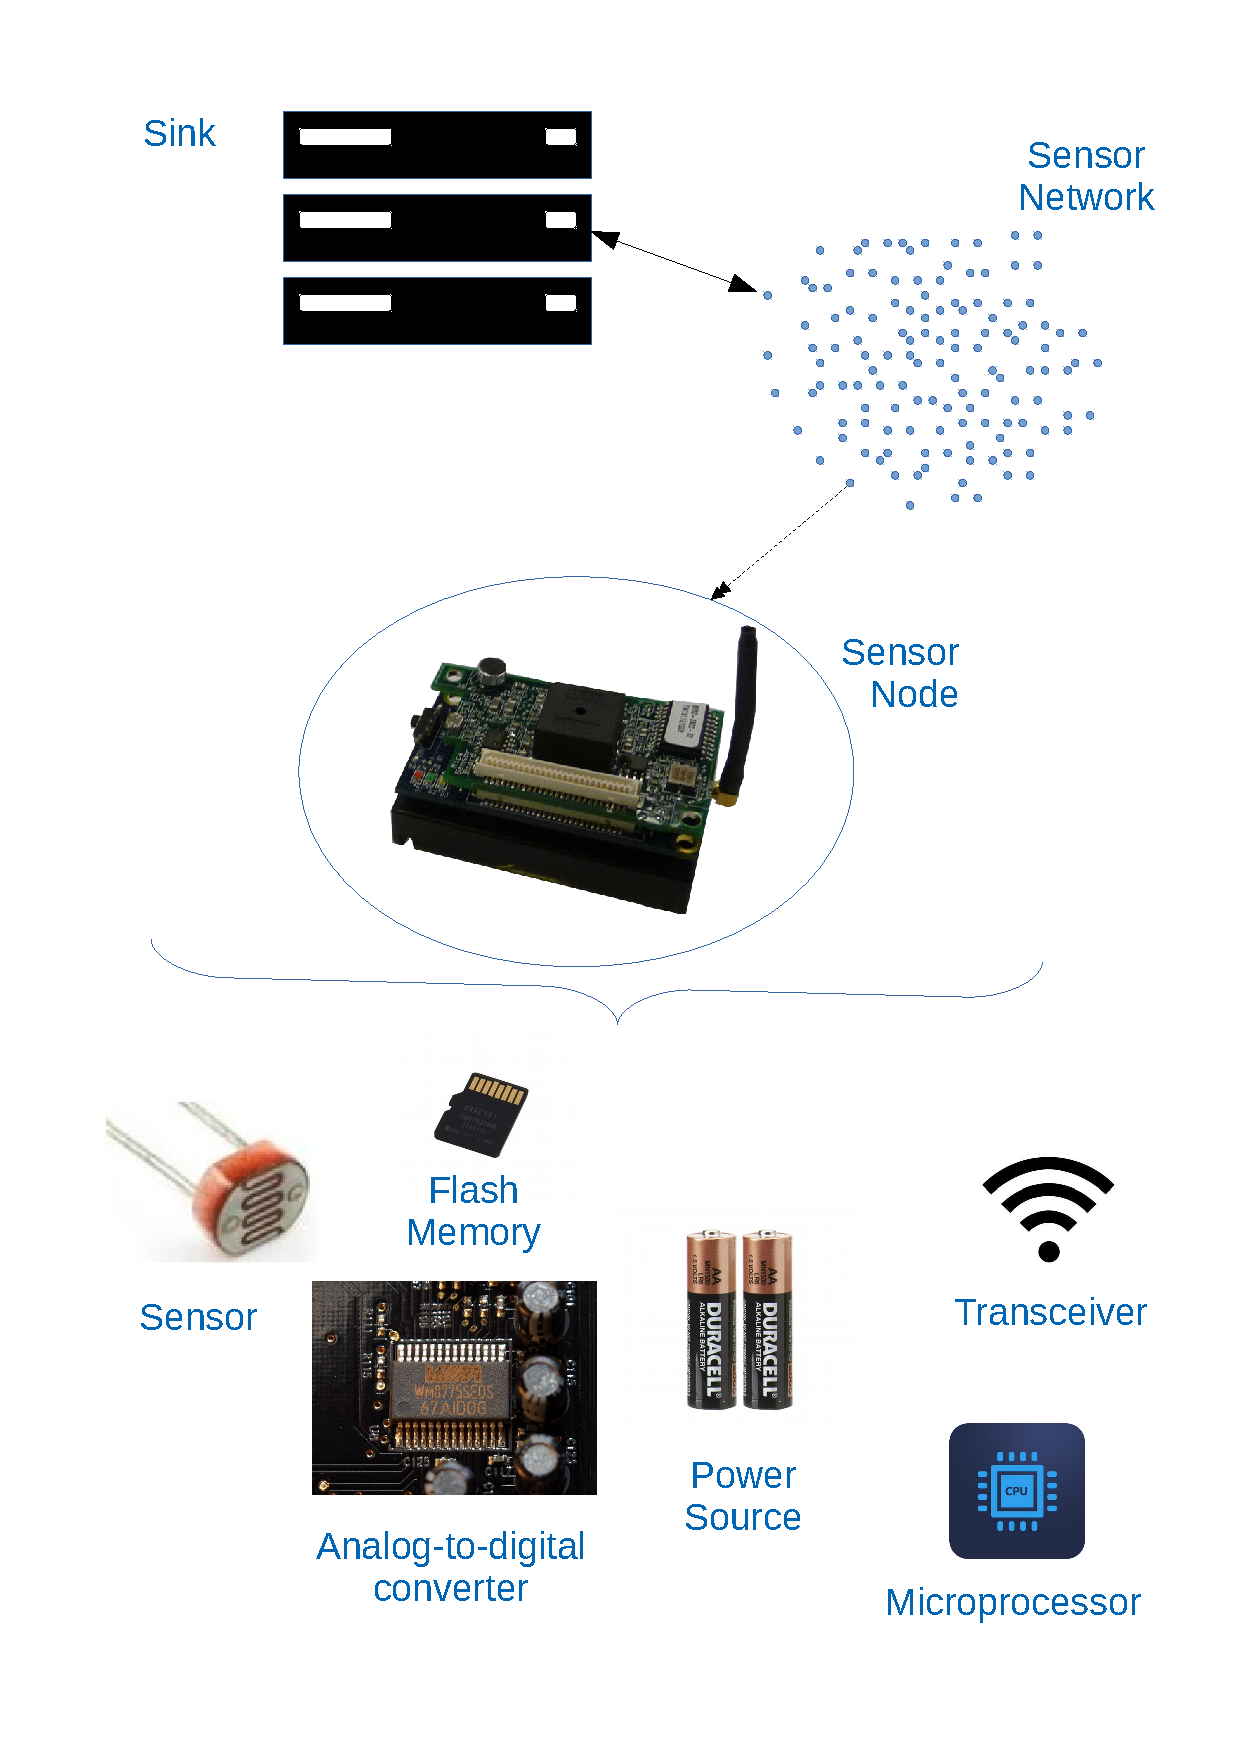
\includegraphics[width=\linewidth, height=0.9\textheight]{images/sensor-network-sensor-node.pdf}
\caption{An illustration of a sensor node in a \ac{WSN}.}
\label{fig:sensor-network}
\centering
\end{figure}

\FloatBarrier

\par
\acp{WSN} and \acp{RSN} are often designed with some sensor nodes sensing the
phenomenon and one or more sinks where the data is routed to. Based on the type
of topology, e.g., a simple star structure (Fig.~\ref{fig:Star Topology}),
sensed data is forwarded to the sink directly, i.e., in a one-hop manner. More
complex topologies, e.g., tree (Fig.~\ref{fig:Tree Topology}) or connected star
structures, often require to relay sensed data through intermediary sensor
nodes to a sink in a multi-hop fashion, as direct communication paths between
sensing and sink are not always possible~\cite{romer2004design}. 
\par
In more complex topologies with a lot of intermediary sensor nodes, finding the
optimal routing path from the sensor node to the sink is not trivial. With an
increasing number of sensor nodes, the complexity of the computation of the
optimal route increases, as sensor nodes have multiple neighbors from which to
choose the next transmission step. Solving such a problem locally, i.e., sensor
nodes compute the next best step, with additional constraints, e.g., minimizing
energy expenditure and meet the quality of data thresholds can be an unfeasible
task. On the other hand, outsourcing this task to the sink could induce a
significant communication overhead with additional energy expenditure.
Techniques on topology control and route pathfinding will be discussed later in
the thesis.
\par
A survey by Alippi et al.~\cite{alippi2009energy} presents a taxonomy of
adaptive sensing strategies. The authors present, i.a. "adaptive sampling" and
"model based active sensing" algorithms. We extend with our work the area of
sampling with filtering as both processes can run at a sensor node level.
Additionally, we present more algorithms from the areas of \ac{CS} and
\textit{Adaptive Filtering} and give a supplementary overview of
\textit{Routing} and \textit{Topology Control} to expand on the challenges
present in sensor data sampling.

\begin{figure}
\begin{subfigure}{.5\textwidth}
  \centering
  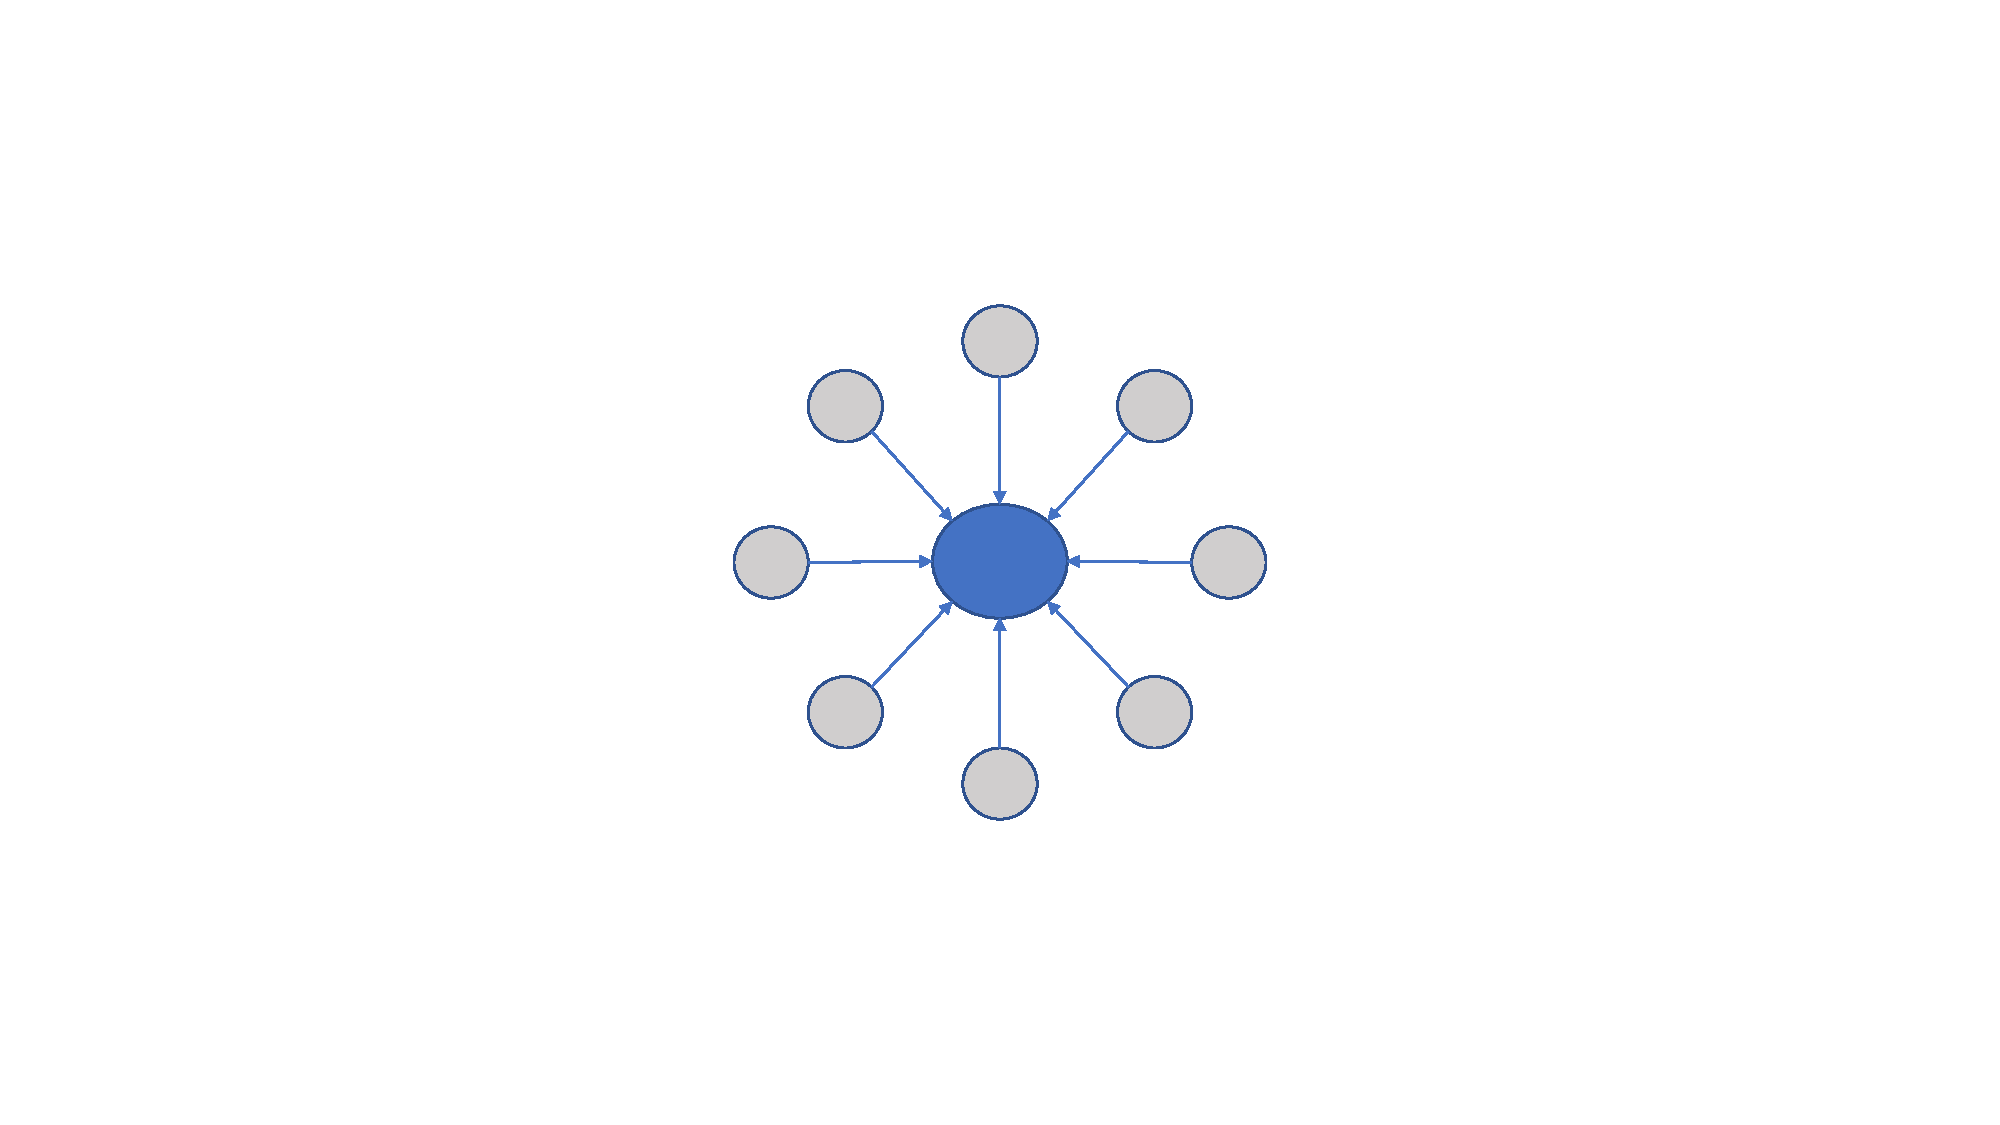
\includegraphics[width=.8\linewidth]{images/star-structure.pdf}
  \caption{}
  \label{fig:Star Topology}
\end{subfigure}%
\begin{subfigure}{.5\textwidth}
  \centering
  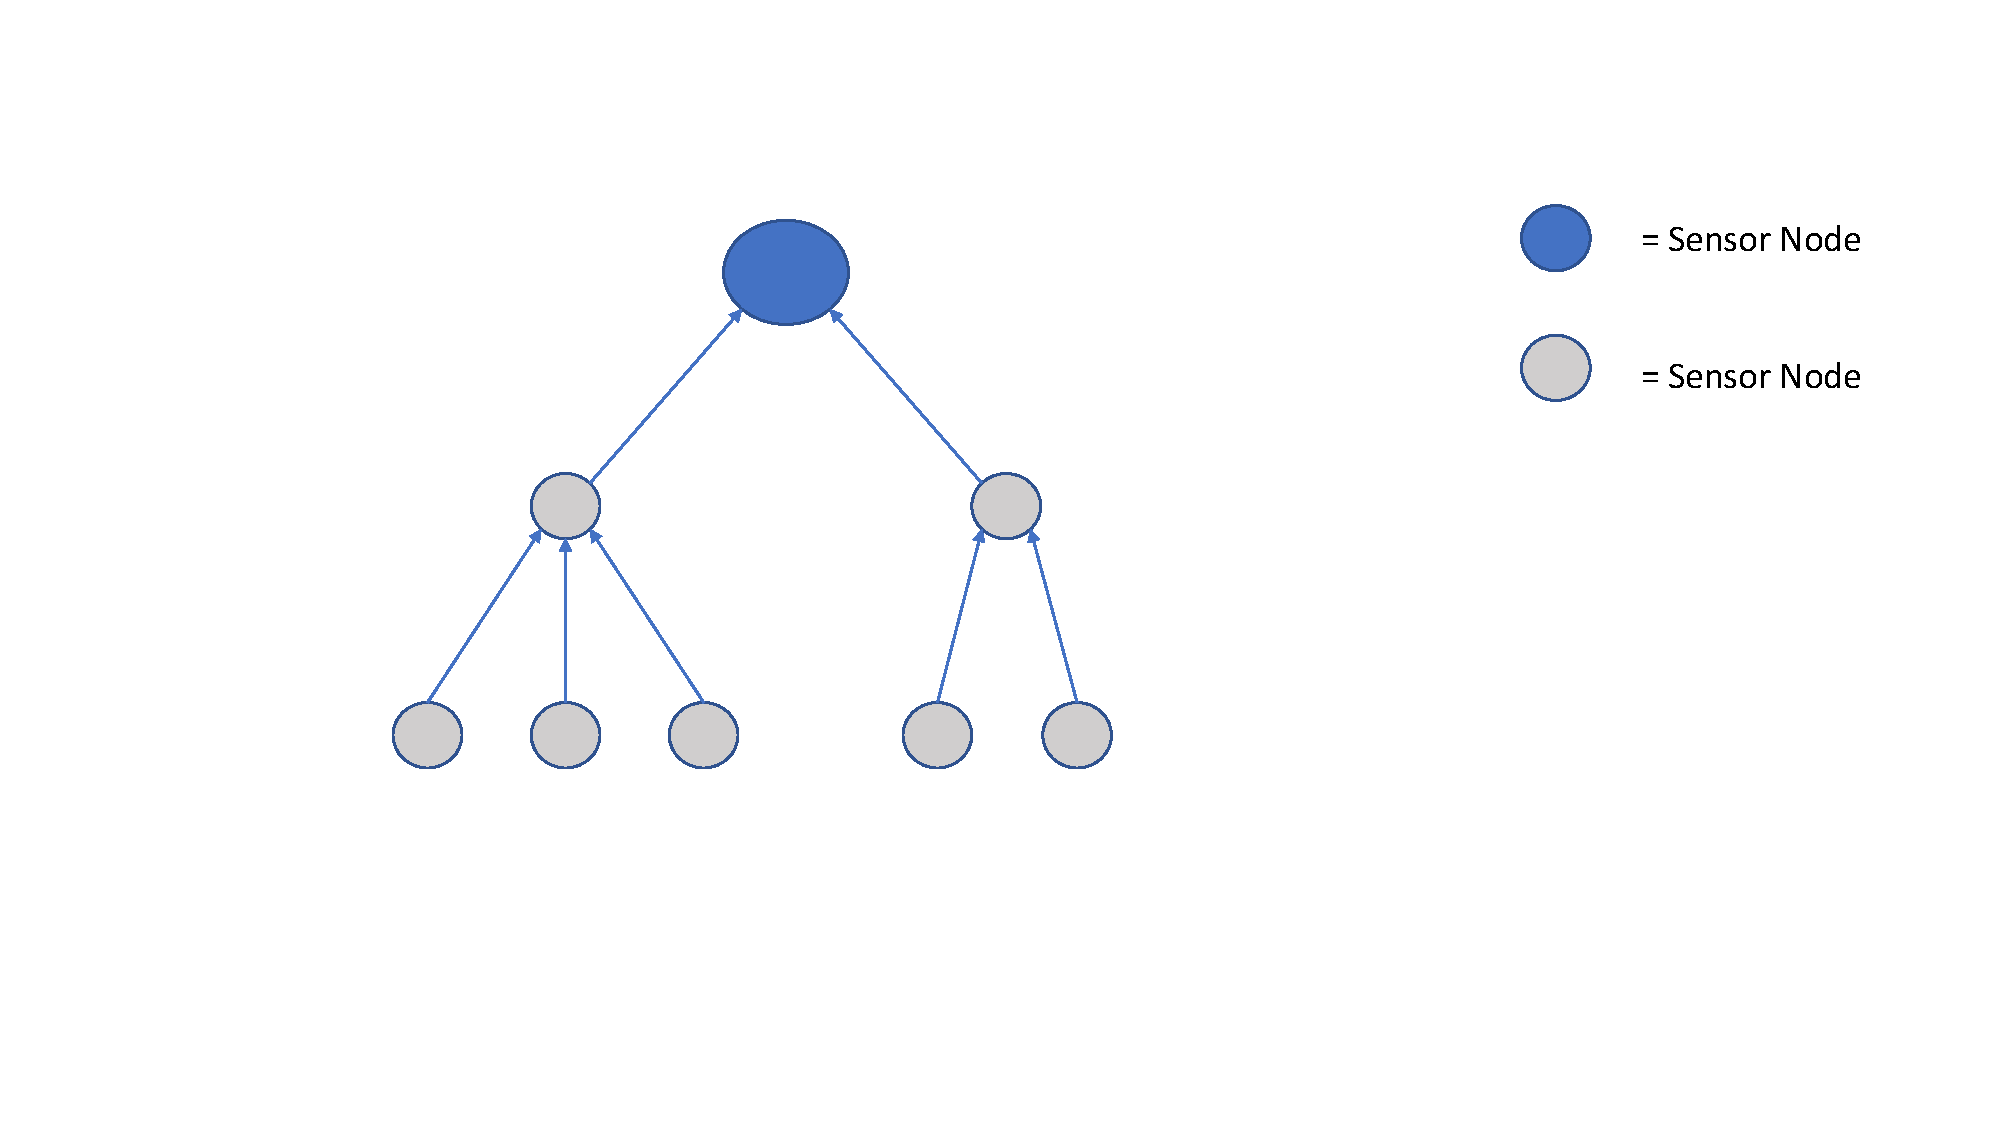
\includegraphics[width=.8\linewidth]{images/tree-structure.pdf}
  \caption{}
  \label{fig:Tree Topology}
\end{subfigure}
\caption{Example Topologies. Inspiration taken from Reina et al.~\cite{reina2013role}}
\label{fig:fig}
\end{figure}

\FloatBarrier


\subsection{Contributions}
\label{sec:contributions}

The contributions of this thesis go as follows: 
\begin{enumerate}
    \item We present a catalog of 15 sampling algorithms for sensor data
    gathering.
    \item We classify the sampling techniques in a taxonomy for a compact
    overview of the field of data sampling in \acp{SN}.
    \item We present relevant information for each algorithm. We summarize
    relevant information as:

        \begin{itemize}
            \item The problem(s) the algorithm tries to solve
            \item Basic workings of the algorithm
            \item Experimental results of the algorithm and how it compares to
            others
            \item Use case(s)
            \item Advantages and limitations of the algorithm
            \item Message Overhead of the algorithm
        \end{itemize}

    \item We present 5 related algorithms from the area of \textit{routing}
    and \textit{topology control}

    \item We present two algorithms which combine techniques from sampling and
    filtering.

    \item We showcase possible combinations of algorithms presented in the
    thesis.

\end{enumerate}

\subsection{Thesis Outline}

\para {Section \ref{sec:Methodology}.}  In section \ref{sec:Methodology}, we
explain our approach in compiling the taxonomy. In
subsection~\ref{sec:Terminology} we define and discuss the terminology used in
this work. Subsection~\ref{sec:Algortihm selection criteria} motivates our
selection criteria for including algorithms in the taxonomy. In
subsection~\ref{sec:Evaluation Metrics} we define our evaluation metrics for
the presented algorithms.

\para{Section \ref{sec:Taxonomy}.}  In section \ref{sec:Taxonomy}, we present a
taxonomy for classifying sampling algorithms. We split the section  into three
subsections.~\ref{sec:Overview} gives an overview of the described classes,
subclasses, and motivations for the classification. Each following section
describes a class and its subclasses in detail. We present relevant information
for multiple algorithms for each subclass. 

\para{Section \ref{sec:Related Algorithms}.} In section \ref{sec:Related
Algorithms}, we review algorithms not covered in the taxonomy from areas other
than sampling, i.e., topology control and routing. We split the section into
three subsections. The subsections~\ref{sec:Routing} and~\ref{sec:Topology
Control} present algorithms from the areas of routing and topology control in
\acp{SN}. In section~\ref{sec:Combination of Algorithms} we discuss possible
combinations of different sampling algorithms.

\section{Methodology}
\label{sec:Methodology}

In this section we present our methodology in conducting our research. This
includes the selection criteria for including algorithms and publications into
the taxonomy and the evaluation metrics for the presented algorithms. We also
include a terminology subsection, where we discuss and define different terms
used in the area of data sampling and \acp{SN}.

\subsection{Terminology}
\label{sec:Terminology}

The literature related to data sampling from sensors defines many different
terms such as data collection (e.g.~\cite{laiymani2013adaptive, liu2007energy,
wang2012adaptive}), data sampling (e.g.~\cite{willett2004backcasting,
jain2004adaptive, szczytowski2010asample}), data gathering
(e.g.~\cite{wang2012data, luo2009compressive, zhang2016data}), and data sensing
(e.g.~\cite{padhy2006utility, mahmudimanesh2012balanced, duarte2005joint}).
Some publications use these terms as synonyms while other publications use
different terms to differentiate concepts. In the following paragraphs, we,
i.a. discuss the definitions of data collection, data sampling, data gathering,
and data sensing. We include this subsection because we need to clarify the
terminology in order to be precise in the following sections. We define other
terms used in this paper, as well. We generally follow the definitions listed
in this section. For words which we identify as synonyms, we decide for one
term and use this term throughout the thesis.

\begin{description}

    \item[Data Stream]
        Hirzel et al.~\cite{hirzel2014catalog} define data streams as "a
        conceptually infinite sequence of data items".

    \item[Network Utilization]
        The standards for technology in automotive retail organization define
        network utilization as "the amount of traffic on the network compared
        to the peak amount that the network can support"~\cite{networkutil}.

    \item[Sensor Node]
        Healy et al.~\cite{healy2008wireless} define sensor nodes as a "[...]
        tiny, cheap, disposable and self contained battery powered computer".
        Sensor nodes usually consist of a processing unit, a communication
        device (sometimes called radio in this thesis), and a sensing
        unit~\cite{akyildiz2002wireless}. We refer to a sensor node "death" if
        it runs out of energy.

    \item[Base Station, Fusion Center, Sink, Sink Node]
        Base station~\cite{padhy2006utility}, fusion
        center~\cite{willett2004backcasting}, sink~\cite{alippi2009energy} and
        Sink Node~\cite{chen2013sink} refer to a computer which is usually
        wired and not restricted in ressources (e.g. CPU, memory, battery).
        We will use the term sink throughout the thesis.

    \item[Centralized Exact, Baseline Transmission Scheme, Naive Scheme]
        Centralized exact~\cite{gedik2007asap}, baseline transmission
        scheme~\cite{luo2009compressive} and naive
        scheme~\cite{cheng2010efficient} all refer to a scheme in which sensor
        nodes report their sensor readings each $ t $ time units without any
        suppression. We will use the term centralized exact throughout the
        thesis.

    \item[\ac{MAN}]
        The \ac{IEEE} defines \ac{MAN} as "a computer network, extending over a
        large geographical area such as an urban area and providing integrated
        communication services such as data, voice, and video"~\cite{ieee802}.

    \item[\ac{LAN}]
        The \ac{IEEE} defines \ac{LAN} as "a computer network, located on a
        user’s premises, within a limited geographical area".~\cite{ieee802}.

    \item[\ac{MAC}-Protocol]
        The \ac{IEEE} defines the \ac{MAC}-protocol as "The protocol that
        governs access to the transmission medium in a \ac{LAN} or \ac{MAN}, to
        enable the exchange of data between \ac{LAN} or \ac{MAN}
        stations"~\cite{ieee802}. This definition is also applicabble to
        \acp{SN}, where the \ac{MAC}-Protocol "coordinates nodes' access to the
        shared wireless medium"~\cite{kredo2007hybrid}.

    \item[Overhead]
        Kabara et al. define [Control Frames] Overhead as "All frames
        containing protocol information and not application data. Energy for
        transmitting and receiving these frames is considered to be
        wasted"~\cite{kabara2012mac}. We denominate control frames overhead as
        message overhead or just overhead in the thesis for reasons of
        breivity.

    \item[Control Message]
        We define control messages as communication between sensor nodes and
        sinks which are not aimed at routing sensed data.

    \item[Broadcasting]
        Broadcasting is a form of information transmission and is employed in
        wireless channels~\cite{lee2013energy}. Broadcasted messages can be
        received by any receiver which is in range.

    \item[Neighboring Sensor Node]
        Two sensor nodes are neighbors if the broadcasted messages of one
        sensor node can be received by the other sensor node. 

    \item[Overhearing]
        Ye et al.~\cite{ye2004medium} define overhearing as nodes picking up
        packets destined for other nodes. They define overhearing as energy
        wasteful, as it consumes energy.

    \item[Multi-Hop]
        Multi-hop routing usually refers to sensor networks in which sensor
        nodes do not communicate directly to sink, but to a neighboring sensor
        node~\cite{yaacoub2012multihop}. The neighboring sensor node then
        communicates to another neighbor or the sink.

    \item[Single-Hop]
        Single-hop topologies are networks in which all sensor nodes can hear
        each other~\cite{ye2004medium}.

    \item[Duty Cycle]
        Lin et al.~\cite{lin2004medium} define a duty cycle as "the ratio of
        the listen interval to the frame length". 

    \item[Duty Cycling]
        Buettner et al defines duty cycling.~\cite{buettner2006x} as an
        approach in which "each sensor node periodically cycles between an
        awake state and a sleep state".

    \item[Sampling Rate, Sampling Frequency]
        The federal agencies digital guidelines initiative defines sampling
        rate or sampling frequency as "the number of samples per second (or per
        another unit) taken from a continuous signal to make a discrete or
        digital signal"~\cite{samplingrate}. We will use the term sampling rate
        exact throughout the thesis.
 
    \item[Sampling Period]
        The University of Amsterdam~\cite{samplingperiod} defines the sampling
        period as "the time difference between two consecutive samples in a
        sound. It is the inverse of the sampling frequency". We apply this
        definition to any signal.

    \item[Data collection and data gathering] 
        Data collection is often mentioned in connection with the whole process
        of acquiring data through sensors in \acp{SN}. A sampling algorithm
        samples a data stream produced by a sensor sensing a phenomenon. The
        data is then routed through the network to the destination. The work of
        Yao et al.~\cite{yao2015edal} contributes, i.a., a technique, for
        finding the lowest cost path for sent data packages in a \acp{WSN}
        while additionally employing compressive sampling. The authors use data
        collection to define this process. Additionally, a survey by Di
        Francesco et al.~\cite{di2011data} defines the term data collection as
        the process of getting data from a sensor node to the sink.
        Vukobratovic et al.~\cite{vukobratovic2010rateless, zhang2016data}
        describe data gathering as the process of collecting and transmitting
        sensed data from sensor nodes to sink. We will use data gathering and
        data collection as synonyms as they both describe the whole process of
        acquiring data at sensor nodes and routing them to a sink.

    \item[Data sensing and data sampling] 
        The definitions for data sampling and data sensing are also inconsistent
        in the literature. Zhao et al.~\cite{zhao2016cats} employ sampling in
        the context of sink assigning sampling tasks, which consist of a time
        window and a sampling period, to sensor nodes. Trihinas et
        al.~\cite{trihinas2015adam} also do not differentiate between sampling
        and sensing.  Aquino et al.~\cite{aquino2014musa} on the other hand,
        discern sensing as the process of a preconfigured sensor unit measuring
        a physical phenomenon and sampling as the software taking samples form
        the data generated by the sensor unit. The distinction is important as
        the authors point out that generally, an online reconfiguration of the
        sensor sensing times is not possible. Contrary, software is more
        flexible and sampling rates and intervals can be specified online.
        However, Deshpande et al.~\cite{deshpande2004model} argue, that a
        sensor can only provide \textit{samples} of an observed, continuous
        phenomenon. Therefore, additional sampling by an algorithm would be
        interpreted as filtering. To stay consistent with our differentiation
        between sampling and filtering, we will not distinguish sampling and
        sensing unless a presented work makes the distinction, e.g., an
        off-the-shelf sensor unit has a fixed sensing rate and can only be
        turned on or off. In such cases, the sampling is done on the data
        stream. Because sensor nodes have only limited
        memory~\cite{akyildiz2002wireless}, only \textit{samples} of the data
        stream would be stored at each point in time, on which additional
        filtering would be applied. Elsewise we use data sampling throughout
        the thesis.

    \item[Stream Sampling]
        Another distinction we would like to make is stream sampling and
        reservoir sampling. Lahiri et al.~\cite{Lahiri2009} define stream
        sampling as "the process of collecting a representative sample of the
        elements of a data stream." The authors further elaborate that stream
        sampling differs from conventional sampling in that data which is not
        sampled when it arrives is lost. \textit{Reservoir Sampling} is an
        instance of stream sampling. 

        % TODO Reservoir Sampling definition finden und zu stream sampling
        % abgrenzen


\end{description}
\par

\subsection{Algortihm Selection Criteria}
\label{sec:Algortihm selection criteria}

Many of the algorithms in our taxonomy focus on \acp{WSN}, which are heavily
constricted in terms of energy, memory and computational power. As such, the
goal of the algorithms is to increase the network lifetime by reducing energy
expenditure, induced by sampling the sensor and communicating the values. We
argue, that many algorithms presented in this thesis can be used outside of
\acp{WSN}. The reduction of data routed through a network, without significant
loss of information, is crucial for applications which produce a lot of data at
high speeds.

We selected the algorithms the taxonomy based on the following criteria:

\begin{itemize}
    \item Algorithms which are associated with each other.
    \begin{itemize}
        \item It is interesting to see, how an algorithm evolves, as authors
        expand on an algorithm or incorporate ideas from that algorithm into
        their work.
    \end{itemize}
    \item Algorithms which highlight different design areas of \acp{SN}
    \begin{itemize}
        \item For example, Jain et al.~\cite{jain2004adaptive} concern
        themselves with wired sensor networks, while Srbinovski et
        al.~\cite{srbinovski2016energy} design their algorithm for \acp{RSN}.
        We found diversity in the use cases interesting.
    \end{itemize}
    \item Algorithms which employ techniques from areas other than distributed
    systems. 
    \begin{itemize}
        \item In our opinion the most representative example is
        \textit{compressive sampling} which uses findings from the domain of
        signal processing to greatly reduce data sent through the network.
    \end{itemize}
\end{itemize}

\subsection{Evaluation Metrics}
\label{sec:Evaluation Metrics}

To provide a better overview of the presented algorithms, we summarize our
findings in table~\ref{table:algorithm table}. A
set of properties describes each algorithm:

\begin{description}
    \item[Assumptions]
        The algorithms presented in the taxonomy assume specific characteristics
        of a sensor network they are deployed in or a signal they observe. We
        sum up the main assumption of an algorithm in the table. We define the
        main assumption as a prerequisite, without which the algorithm cannot
        perform the way the authors of the algorithm intended.
    \item[Advantages]
        We present the advantages of an algorithm as the authors define them.
        Given that many of the presented algorithms position themselves as
        energy efficient, we do not include energy efficiency as an advantage.
        Rather, we include algorithm traits which make an algorithm stand out
        more in its strengths. However, the presented traits are not distinct,
        as algorithms, especially from the same category, share strengths and
        weaknesses (e.g., \textit{EDCA} and \textit{STCDG} share many
        properties, as \textit{STCDG} is an extension of \textit{EDCA}).
    \item[Limitations]
        Similar to the advantages, we include limitations of algorithms as the
        authors or authors of other work define them. 
        % Limitations can be in terms of use cases, i.e., an algorithm is not
        % suitable for large-scale sensor networks, or 
    \item[Message Overhead]
        We added message overhead as an algorithm property because overhead
        generated through communication between sensor nodes or the sink
        concerns all types of networks. Overhead, e.g., control messages sent by
        a server to a sensor node, demands allocation of bandwidth which loads
        the network and can lead to message delays. We define different levels
        of message overhead:

        \begin{itemize}
            \item \textit{Low}. A low message overhead is present if the sensor
            nodes work autonomously, i.e., no control messages are sent by the
            sink, after an initial "set-up" phase in which a sink configures
            parameters at sensor nodes. Communication between sensor nodes is
            limited to multi-hop routing.

            \item \textit{Medium}. Algorithms with a medium message overhead
            allow sensor nodes to work independently from one another, with the
            exception of communicating to and overhearing messages from
            neighboring sensor nodes.

            \item \textit{High}. High message overhead is present if
            algorithms require the sink to periodically make adjustments to
            the configuration of sensor nodes or the network in general.
        \end{itemize}

        The message overhead of an algorithm, which is "in between" a level, is
        elaborated on in the taxonomy.

        The properties of the algorithms presented in the table, except for
        \textit{communication overhead}, are statements from the authors of the
        algorithm or analysis of other authors. If no reference is given, then
        the statement is from the author of the algorithm.

\end{description}


\section{Taxonomy}
\label{sec:Taxonomy}

In this section, we present our taxonomy of sampling algorithms for \acp{SN}.
We classify algorithms into two categories: \catI (Section~\ref{sec:catI}) and
\catII (Section~\ref{sec:catII}). \catI are all algorithms which prevent the
\textit{sampling} of redundant data. This is achieved at the sensor node level,
manipulating the sampling rate to capture all relevant information from a data
stream produced by a sensor. In contrast, \catII focus on suppressing already
sampled data by utilizing spatial and temporal correlations between sampled
values. We decided to include \catII into the taxonomy, as filtering and
sampling both take place at the sensor node level and are applied before data
is sent to data consumers.

\subsection{Overview}
\label{sec:Overview}

We visualize our taxonomy in Fig.~\ref{fig:Taxonomy}.

\begin{figure}[h]
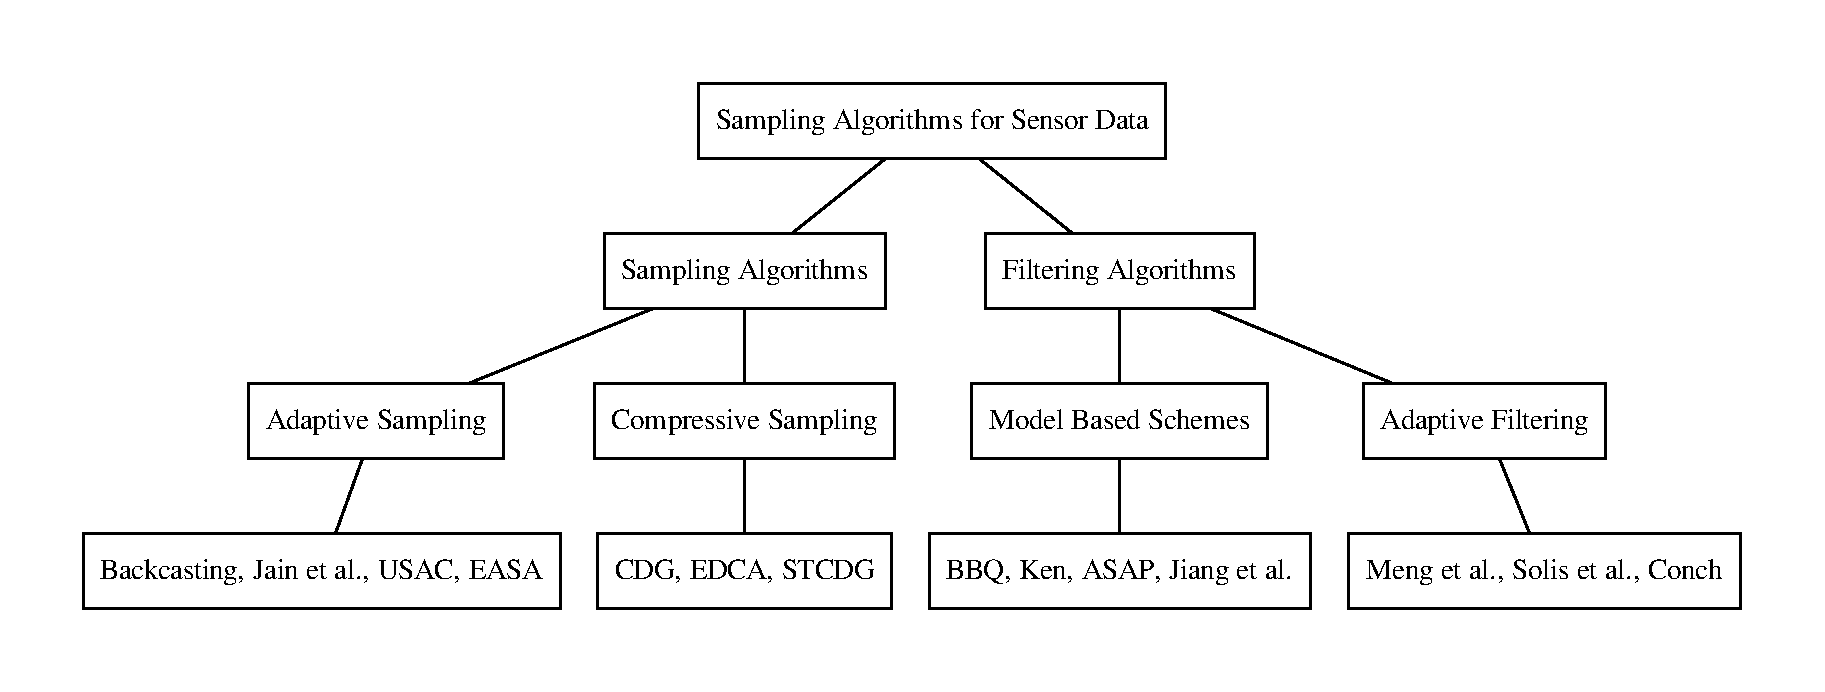
\includegraphics[width=\linewidth]{images/taxonomy.pdf}
\caption{Taxonomy of the presented Algorithms}
\label{fig:Taxonomy}
\centering
\end{figure}

% \FloatBarrier
% 14 algs

The presented algorithms are summed up and compared in
table~\ref{table:algorithm table}. We will address the algorithms by the names
the authors have given them and additionally reference the paper. If the
algorithm has no name, the authors are referenced instead.

% \begin{table}
    % \begin{adjustbox}{angle=90}
        % \bgroup
        \def\arraystretch{1.5}%
        \begin{longtable} { |p{.20\textwidth}||p{.20\textwidth}|p{.20\textwidth}|p{.20\textwidth}|p{.10\textwidth}| } 
            % { |p{3.5cm}||p{3cm}|p{3cm}|p{3cm}|p{2.5cm}| } % { |c||c|c|c|c| }

        \hline
        Algorithm & Assumptions & Advantages & Limitations & Message Overhead\\
        \hline
        \hline

        \textit{Backcasting}~\cite{willett2004backcasting} & Spatial and
        temporal correlation of the signal. & Random sensor deployment. &
        Premature death of cluster heads. & High\\ % \hline

        Jain et al.~\cite{jain2004adaptive} & Sensor data is streamed
        continiously & Important data receives more bandwidth & Only Single-hop
        \acp{SN} & High\\ % \hline

        \textit{USAC}~\cite{padhy2006utility}& Fix number of sensor nodes &
        Captures sudden changes in data & Static confidence
        interval~\cite{kho2007decentralised} & Low\\ % \hline

        \textit{EASA}~\cite{srbinovski2016energy}& Sensing consumes more energy
        than communicating & Adaptive to energy levels & Complex computation &
        High\\ % \hline

        \textit{CDG}~\cite{luo2009compressive}& Knowledge of domain in which
        observed signal is k-sparse & Low packet loss & Not suitable for small
        scale \acp{SN} & Low\\ % \hline

        \textit{EDCA}~\cite{cheng2010efficient}& Matrix of collected values
        exhibits low-rank feature & Robust against packet loss & Empty columns
        reduce recovery accuracy~\cite{cheng2013stcdg} & Low\\ % \hline

        \textit{STCDG}~\cite{cheng2013stcdg}& low-rank and short term stability of
        matrix & Adaptible since independent of \ac{SN}-type & Not suitable for
        small scale \acp{SN}~\cite{yi2015partial} & Low\\ % \hline

        \textit{BBQ}~\cite{deshpande2004model}& Slow topology change & Exploits
        correlation between sensor and voltage levels & Not suitable for
        anomaly detection & Low\\ % \hline

        \textit{Ken}~\cite{chu2006approximate}& Slow topology
        change~\cite{gedik2007asap} & Suitable for anomaly detection &
        Prediction Models constructed at sink~\cite{gedik2007asap}  &
        Medium-High~\cite{gedik2007asap}\\ % \hline

        \textit{ASAP}~\cite{gedik2007asap}& Forgo some data quality for less
        energy expenditure & In-network construction of models and clusters &
        Not suitable for anomaly detection & Low\\ % \hline

        Jiang et al.~\cite{jiang2011prediction}& Forgo some data quality for
        less energy expenditure & Prevents energy costly and inaccurate
        predictions & not suitable for anomaly detection & Low\\
        % \hline

        Meng et al.~\cite{meng2004event}& Events are sensed by more than one
        sensor & Suppression is computationally simple & Relative difference of
        sensor readings not leveraged~\cite{silberstein2006constraint}& Medium\\
        % \hline

        Solis et al.~\cite{solis2005efficient}& Spatial correlation of sensor
        readings & Simple computation at sensor nodes & No contour map
        calculation given~\cite{xu2008cme} & Medium\\ % \hline

        \textit{Conch}~\cite{silberstein2006constraint}& Spatial and temporal
        correlation of signal & Flexibility to increase network robustness or
        energy efficiency & Sensor Nodes must know network
        topology~\cite{trihinas2017admin}& Low\\ % \hline

        \textit{CME}~\cite{xu2008cme} & Stationary sensor nodes & Good
        scalability~\cite{khelil2014comparative} & Premature death of cluster
        heads~\cite{khelil2014comparative} & Medium\\

        \hline
        \caption{Table of presented Algorithms}
        \label{table:algorithm table}
        \end{longtable}
        % \egroup
    % \end{adjustbox}
% \end{table}

\FloatBarrier


\subsection{\catI} % Sampling Algorithms
\label{sec:catI}

The first category of our taxonomy incorporates all algorithms which primary
focus lies on manipulating the sampling rate of one or multiple sensor nodes to
reduce network utilization. Although there are algorithms from other categories
which also may incorporate manipulations to the sensing/sampling rates of
sensor nodes (e.g.~\cite{trihinas2015adam, chatterjea2008adaptive}), we include
algorithms to the Sampling Algorithms category only if the main focus of the
work lies on sampling rate manipulation. 

In our research we found adaptive sampling and compressive sampling to be good
sub classifications for sampling algorithms. Both types of algorithms target
sampling rates of sensor nodes to reduce network traffic. Adaptive sampling
algorithms employ schemes to dynamically react to changes in the behaviour of
an observed phenomenon, by manipulating sensing rates of sensor nodes.
Compressive sampling utilizes findings from the field of signal processing, to
sample signals, i.e. data streams from an observed phenomenon, below the
typical Nyquist rate~\cite{candes2008introduction}. From such a subset of data,
the original signal can be reconstructed at sink with very high accuracy.

\subsubsection{Adaptive Sampling}
\label{sec:Adaptive Sampling}

Trihinas et al.~\cite{trihinas2015adam} define adaptive sampling as:

\begin{quote}
    "The process of dynamically adjusting the sampling rate to the current
    metric evolution, such that when stable phases in a metric stream are
    detected, the sampling rate is reduced to ease processing and energy
    consumption."
\end{quote}

\par
\textit{1) Backcasting:}
Although the quote is from 2015, the idea of adaptive sampling goes back to the
2000s. One technique called \textit{Backcasting} was presented by Willet et
al.~\cite{willett2004backcasting}. The key idea of the work is that a monitored
environment exhibits correlations in time and space domains which can be
exploited to reduce the number of required sensor nodes to deliver an accurate
picture about the monitored environment. The authors assume that the sensor
network is a rectangular field of uniformly distributed sensor nodes.
Initially, a subset of the sensor nodes is chosen by the sink to provide an
initial estimate of the sensed phenomenon by a \ac{RDP}. Singh et
al.~\cite{singh2006active} describe a \ac{RDP} as being identifiable "with a
tree structure, where each leaf of the tree corresponds to a cell of the dyadic
partition." A subset of nodes are multiple clusters of nodes with a cluster
head each. Cluster heads route the data from the sensor nodes to the sink and
vice versa. The sink receives the sensed data and activates additional nodes to
improve the quality of the sampling by reducing the \ac{MSE}. However, this
leads to additional message overhead as control messages have to be routed
through the network. The authors evaluate their approach theoretically and
conclude, that a \ac{WSN} with 10000 sensors and energy to operate continuously
for a year, would run for ten years when using \textit{Backcasting}. The
authors point out that the network lifetime could be improved if mechanisms for
cycling the position of cluster head would be implemented. Although the
algorithm does not manipulate the sampling rates of individual sensor nodes, it
is still one of the first algorithms to adaptively change the sensing tasks of
nodes based on the dynamics of the observed phenomenon.

\par

\textit{2) Jain et al.:}
Another technique, also from 2004, was published by Jain et
al.~\cite{jain2004adaptive}. The authors' main contribution is an algorithm to
change the sampling rate of individual sensor nodes in a stream sensor network
based on the importance of the observed data. An important event could be a
camera observing non-standard driving behavior of a car, e.g., driving in an
erratic course or a temperature spike in a data center. At the sensor node
level, Kalman filters predict sensed values. They are then compared against the
actual sensed values. The values are stored in a sliding window locally. An
estimation error is computed over the sliding window. The estimation error
indicates a changing dynamic of an observed phenomenon. After each taken
sample, a sensor node adjusts its \ac{SI}, i.e. the time interval between two
consecutive samples. If the desired \ac{SI} lies in the \ac{SIR}, the sensor
node can change its \ac{SI} locally. Otherwise, the sensor node has to request
a new \ac{SI} from the sink. The sink keeps a metric of available communication
resources which gets updated after a request to change a \ac{SI} is accepted.
The requests are stored in a job queue. To approve a \ac{SI} a linear
optimization problem has to be solved. The additional communication with the
sink induces a high message overhead. The authors evaluated their approach on
synthetic data generated by a spatiotemporal data generator. Tested metrics
where the mean fractional estimation error $ \eta $, the proportion of messages
exchanged between the source and the sink and the number of values sensed by
the source nodes \textit{m}. The adaptive sampling algorithm outperformed the
alternative uniform sampling algorithm almost in every test. Tests were done,
i.a using different numbers of sensor nodes and sliding window sizes. The
authors indicate that the algorithm does not apply to multi-hop sensor
networks, i.e., a sensor node has to have a direct connection to the sink.
Furthermore, both the sliding window and the \ac{SIR} have to be chosen by the
user. Also, the authors state that the message overhead is high. The main goal
of the algorithm is to optimize bandwidth usage in the network, thus this
technique is more suitable for wired \acp{SN} and less for \acp{WSN} as the
communication overhead is high, and communication consumes a major amount of
energy in most sensor nodes~\cite{raghunathan2002energy}.

\par

\textit{3) \ac{USAC}:}
A technique designed initially for a glacier monitoring application by Padhy et
al. \ac{USAC}~\cite{padhy2006utility} is an example of an adaptive sampling
scheme for a \ac{WSN}. The algorithm uses a linear regression model at each
sensor node to capture phase shifts of the observed phenomenon as fast as
possible. The model predicts values at a sensor node. Those values are checked
against the actual sensed values. If a predicted value lies in the user-defined
\ac{CI}, then the sensor node reduces its sampling rate by a multiplicative
factor $ \alpha $ until the sampling rate reaches $ f_{min} $. The user sets $
f_{min} $. If the value does not lie in the \ac{CI}, then the sensor node
raises its sampling rate to $ f_{max} $ to capture a supposed change in the
dynamic of the observed phenomenon. No additional communication happens with
the sink. The experiments tested the algorithm against the older deployed
protocol in the glacier monitoring application \textit{GLACSWEB}. In the
\textit{GLACSWEB} protocol, sensor nodes send their data directly to the sink.
This technique is energy inefficient as the authors state that
\begin{quotation} "(...) the power required to transmit data from one node to
another is proportional to the square of the distance between the nodes (...)."
\end{quotation}

Additionally, \textit{GLACSWEB} has a static sampling rate which the authors
argue, induces unnecessary sampling.

The tests were conducted in a simulated environment using historical data from
the application. The authors tested different network topologies, numbers of
sensor nodes in a network and the number of changes in the dynamic of the data.
The experiments resulted in \ac{USAC} outperforming the older algorithm in
every test. The efficiency increase, which is defined by the authors as

\begin{quotation}
    "The value of the data gained over the energy consumed of USAC relative to
    GLACSWEB in each case."
\end{quotation}


was, i.a. 470\% when distributing sensor nodes randomly around a central base
station.
\par

\textit{4) \ac{EASA}:}
\acp{RSN} combine the perpetual operation lifetime of wired \acp{SN} and the
flexibility of \acp{WSN}. However, \acp{RSN} introduce new challenges for
designing data collection algorithms. A paper from Srbinovski et
al.~\cite{srbinovski2016energy} presents an adaptive sampling algorithm for
\acp{RSN} with energy-hungry sensors. The authors point out, that contrary to a
common assumption that communication consumes most of the energy in sensor
nodes (e.g., ~\cite{santini2006adaptive}), the sensor unit can be the main
energy consumer~\cite{boyle2012energy}. The authors contribute an \ac{EASA} for
perpetually operating \acp{RSN} which builds upon the \ac{ASA} by Alippi et
al.~\cite{alippi2007adaptive}. The \ac{ASA} algorithm leverages the Nyquist
Theorem $$ F_N > 2 \cdot F_{max} $$ for finding the optimal (minimum) sampling
rate $ F_N $. To estimate the maximum frequency in the power spectrum $ F_{max}
$, a \ac{FFT} is used on the first $ W $ samples of the process. A \ac{CI} can
be defined to capture changes in the dynamic of the process. The algorithm is
run on the sink due to computational complexity; thus message overhead is
present. \ac{EASA} expands \ac{ASA} with energy awareness, i.e., adjusting the
optimal sampling frequency of a sensor node based on current and critical
battery level, and rate of energy saving. When the battery level drops below
the user-defined critical value $ m $, the sampling rate deviates from the
optimal \ac{ASA} sampling rate. This may lead to the sensor not capturing the
signal fully as the Nyquist theorem is violated. The authors argue that a
potential loss in data quality is the cost of staying continuously in the
network. The authors tested \ac{EASA} extensively on data from two deployments.

\begin{enumerate}
    \item A custom, wind-powered deployment for measuring wind speed
    \item An off-the-shelf solar powered deployment for measuring $ CO_2 $ in a
    beehive
\end{enumerate}

\ac{EASA} was tested with different saving rates against \ac{ASA} and
additionally on the second deployment against a fixed rate. All tests were done
in a simulated environment. In both deployments, \ac{ASA} and \ac{EASA} have
the same sampling rate when the battery level is above $ m $. \ac{ASA} can
deliver a high data quality, as the sampling rate is always optimal. \ac{EASA}
on the other hand, stabilizes in the first deployment the energy levels of the
sensor node after 36 days of operation at $ 60\% $ with a $ m $ of $ 1/3 $.
With \acp{ASA} the energy levels are at $ 20\% $. In the second deployment,
\ac{ASA} gets outperformed slightly in energy consumption by \ac{EASA}. The
energy levels with the fixed sampling rate are depleted after 13 days.

% Adaptive Monitoring by Tata and MEGAhed. Goal: Determine metrics which should
% be monitored and the frequencies with which they should be monitored. 


\subsubsection{Compressive Sampling}
\label{sec:Compressive Sampling}
\ac{CS} is a relatively new sampling paradigm which was first introduced by
Donoho et al.~\cite{Donoho06compressedsensing} in 2006. Mahmudimanesh et
al.~\cite{mahmudimanesh2010reordering} describe \ac{CS} as:

\begin{quotation}
    "\ac{CS} states that it is possible to reconstruct a discrete signal from a
    set of randomly chosen values selected from a vector computed by a linear
    transform of the discrete signal vector."
\end{quotation}

Candés et al.~\cite{candes2008introduction} summarize the main principles of
\ac{CS} as sparsity and incoherence. A signal is sparse when "[it] contains
only a small number of non-zero elements compared to its
dimension"~\cite{elzanati2015collaborative}. Candés et al. define incoherence
as when a sample of a sparse signal has an "extremely dense" representation in
some domain $ \Psi $~\cite{candes2008introduction}. Luo et
al.~\cite{luo2009compressive} give an example of a signal being sparse in
\ac{DCT} domain in Fig.~\ref{fig:sparsesignal}.

\begin{figure}
\centering
\begin{minipage}{.5\textwidth}
  \centering
  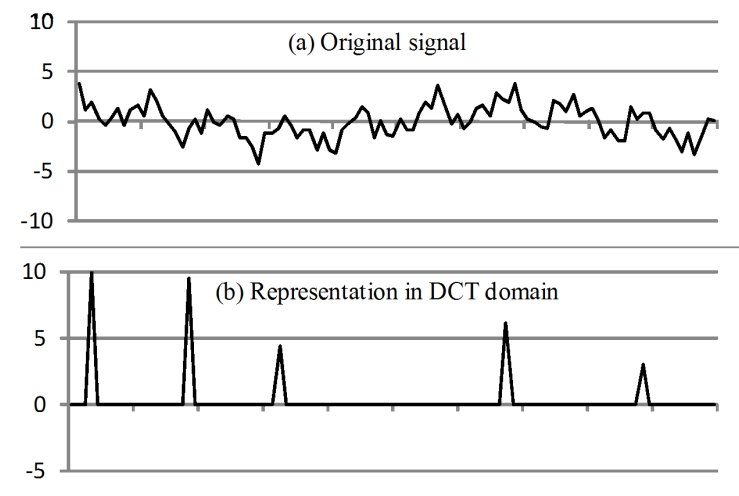
\includegraphics[width=\linewidth]{images/example-signal-sparse.png}
  \captionof{figure}{A sparse signal in the DCT domain~\cite{luo2009compressive}}
  \label{fig:sparsesignal}
\end{minipage}%
\begin{minipage}{.5\textwidth}
  \centering
  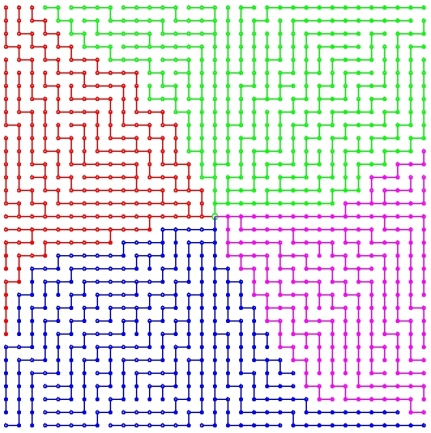
\includegraphics[width=\linewidth, height=5.3cm]{images/grid-topology-luo.png}
  \captionof{figure}{A grid topology~\cite{luo2009compressive}}
  \label{fig:grid topology}
\end{minipage}
\end{figure}

\textit{5) \ac{CDG}:}
Luo et al.~\cite{luo2009compressive} developed a \ac{CDG} algorithm for large
scale sensor networks. The goal of the algorithm is to decrease energy
expenditure and distribute energy consumption evenly across all sensor nodes to
maximize the lifetime of the network. This is achieved by reducing the data
traffic in a network by compressing data readings at each hop. This would lead
to $ M $ messages arriving at the sink from $ N $ sensor nodes, where $ M << N
$. The sink broadcasts a random seed to the network with which each sensor node
can generate, together with its identifier, a local seed. Afterward, no message
overhead is present. Sensor nodes then use the local seed to generate a random
coefficient $ \phi_i $ which they transmit together with their sensor reading $
d_i $ to their parent node. Parent nodes receive readings from their child
nodes and sum up the input with their own $ d $ and $ \phi $. Therefore, every
sensor node transmits only one value. This ensures the sink receives $ M $
weighted sums $ y $, which consist of a matrix of the random coefficients, $
\Phi $ and all sensor readings \textbf{d}:

$$
\begin{pmatrix}
    y_1 \\
    y_2 \\
    \vdots \\
    y_M
\end{pmatrix}
=
\begin{pmatrix}
    \phi_{11} & \phi_{12} & \dotsb & \phi_{1N}\\
    \phi_{21} & \phi_{22} & \dotsb & \phi_{2N}\\
    \vdots & \vdots & \vdots & \vdots\\
    \phi_{M1} & \phi_{M2} & \dotsb & \phi_{MN}\\
\end{pmatrix}
=
\begin{pmatrix}
    d_1 \\
    d_2 \\
    \vdots \\
    d_N
\end{pmatrix}
$$

The random matrix $ \Phi $ is not transmitted because the sink can compute the
matrix if it knows the identification of the sensor nodes. The original sensor
readings \textbf{d} can be reconstructed at the sink by solving:

$$
\displaystyle{\min_{x\in R^N} \ ||x||_{l_1}}  \ \ \   s.t.  \ \  y = \Phi \textbf{d} , \ \ 
\textbf{d}  = \Psi x
$$

$ \Psi $ is the domain in which \textbf{d} can be represented by $ K << N
$ coefficients and $ x $ is the vector of coefficients.

The authors evaluated \ac{CDG} against centralized exact (all nodes transmit as
soon as readings are acquired) with the ns-2 simulation
tool~\cite{bajaj1999improving}. Additionally, testing was done on two real-life
datasets to evaluate the reconstruction capability. For the simulated
environment, the authors created two synthetic sensor networks. The first is a
network with a chain topology, with 1000 sensor nodes spaced 10 meters apart
from each other and with sinks located at each extreme of the chain. The second
set-up was a grid-like routing tree with 1089 sensor nodes and a sink node in
the center of the network, e.g., Fig.~\ref{fig:grid topology}. The authors
varied in their testing runs the signal input intervals and observed the
package loss and output interval change. \ac{CDG} outperformed centralized
exact in both topologies managing input intervals five times and 2.3 times
smaller than the centralized exact in the chain and grid topologies
respectively. Additionally, \ac{CDG} achieved a packet loss of near zero in
both topologies, while the centralized exact had package loss rates of 5\% and
20\% in the chain and grid topologies respectively.

The real-life datasets consist of measurements collected in the Pacific Ocean
by a single moving device and a sensor network in a data center. The authors
argue that the Pacific Ocean dataset has the same properties as data collected
by a sensor network. The authors found the Pacific Ocean data to be sparse in
the wavelet domain. \ac{CDG} can reconstruct the initial 1000 data points from
40 data points with $ > 98\% $ precision. The data points are the 40 highest
coefficients in the wavelet domain of the data. The authors did not find a
sparse representation of the datacenter dataset as the data exhibit little
spatial correlation. Instead, they opted for reorganizing the dataset by
sorting the temperature values in ascending order at the moment $ t_0 $. The
result is sparse in the wavelet domain, and the original signal can be
reconstructed.
\par
\textit{6) \ac{EDCA}:}
One paper by Cheng et al.~\cite{cheng2010efficient} builds upon the low-rank
feature of a matrix. The authors point to discoveries proving that a matrix
formed from spatial and temporal correlated data is approximately low-rank and
can be recovered from a subset of the data~\cite{vuran2004spatio,
candes2009exact}. With the \ac{EDCA} sensor nodes sample at a fixed rate and
send their sensed values to a central sink in a multi-hop scheme. No additional
control messages are sent from the sink to the nodes, except for the
sampling rate. However, the authors point out that missing values, i.e., no
values in some time slots, can be recovered with low error. The focus of the
algorithm lies in the recovery of a low-rank matrix. The authors use the
nuclear norm to solve the rank minimization problem

$$
minimize \ rank(X), \ s.t. \ A(\cdot)=B
$$

where $ X $ is the matrix arriving at the sink and $ A(\cdot) $ is an operator
representing the incompleteness of the matrix. Because the problem is NP-hard,
the authors use a heuristic and shift the problem to a convex optimization
problem

$$
minimize \ || \ A(LR^T) - B \ ||^2_F + || \ L \ ||^2_F \ + || \ R \ ||^2_F
$$

where $ X $ is deconstructed with \ac{SVD} into $ X = U \Sigma V^T $ and $ L =
U\Sigma^{1/2}; \ R = V\Sigma^{1/2}$. The problem is solved using a method by
Zhang et al.~\cite{zhang2009spatio}.

Testing was done using a publicly available dataset of temperature measurements
by sensor nodes from the Intel Berkeley Research lab~\cite{labdata} and a
synthetic dataset. With the real world data, the authors tested the accuracy of
\ac{EDCA} while using different sampling ratios for the 54 sensor nodes. The
authors could only observe small recovery errors. With a sampling ratio of 0.2,
i.e. every fifth sensed value is transmitted, the standard deviation $ \sigma $
was $ < 0.15°C $. With the synthetic data set, the authors compared \ac{EDCA}
with centralized exact, in which all sensed data points are sent to the sink,
on network lifetime. The authors define the lifetime of a sensor network as
"the time duration of the first sensor node which runs out of power." The
lifetime ratio is defined as $ (1/M_{max}) / (1/M_0) $ where $ M_{max} $ is
"the maximum power wasted [...] on every simulation using \ac{EDCA}" and $ M_0
$ the power wasted by centralized exact. The authors found the lifetime ratio
to be 5 when having a sampling ratio of 0.2, increasing the lifetime of a
network fivefold in comparison to centralized exact. 

\textit{7) \ac{STCDG}:}
Another paper by Cheng et al.~\cite{cheng2013stcdg} expands \ac{EDCA} and
introduces a \ac{STCDG} algorithm. Similar to \ac{EDCA}, \ac{STCDG} exploits
the low-rank feature and the short-term stability of data gathered through a
\ac{SN}. The authors argue, that, unlike \ac{CDG}, \ac{STCDG} is more flexible
and does not have to be customized for a specific \ac{SN}. This comes from the
fact, that with \ac{CDG} the domain in which the data is sparse has to be
known in advance. Additionally, \ac{CDG} utilizes only the sparsity of data,
requiring the full dataset to be reordered if the data is not sparse.

The authors deployed a sensor network in a residential building. They used the
data to analyze short-term stability and low-rank of spatially and temporally
correlated data. The authors found the data to have a good low-rank
approximation and short-term stability. Short-term stability is defined by the
authors as the difference between adjacent gaps of sensor readings, with gaps
being the time between two adjacent sensor readings. So the difference is
defined as
$$
dif(n,t) = X(n,t + 1) + X(n,t - 1) - 2X(n, t); \ \ where  \ \ 1 <= n <= N  \ \ and  \ \ 2 <= t <= T - 1
$$
thus, if $ dif(n, t) $ is small then sensor readings at node n around timeslot
t are stable.

The authors expanded their optimization problem formulation to include a tuning
parameter $ \zeta $ to tradeoff fitting the algorithm to the data and achieving
low-rank. With the short term stability added to the optimization problem, as
the difference for all data points in the original matrix $ X $, $
||(LR^T)S^T||^2_F $ the optimization problem is now

$$
minimize \ ||(LR^T). \cdot Q-B||^2_F + \zeta(||L||^2_F + ||R||^2_F) + \eta ||(LR^T)S^T||^2_F
$$

Another extension of \ac{STCDG} is the handling of empty columns. Empty
columns may appear at the sink when the sampling ratio is low, or the packet
loss rate is high. The authors point out that such cases can lead to very high
recovery errors. Therefore, the algorithm ignores empty columns first and
recovers the original matrix. The empty columns are separately filled using the
short-term stability feature. Additionally, abnormal values sensed by sensor
nodes are transmitted independent of the set sampling ratio.

The authors tested \ac{STCDG} against \ac{EDCA} and \ac{CDG} on 3 different
datasets in terms of recovery error, power consumption and network capacity.
The used datasets were the Intel Berkeley Research lab~\cite{labdata} sensor
data, a synthetic trace generated with the ns-2 tool~\cite{bajaj1999improving},
and the residential building data gathered by the authors. Specifically, the
authors subdivided the laboratory and residential building data sets into
singular sensed phenomena, namely light and temperature. \ac{NMAE} was used to
measure the recovery performance of the algorithms. The researchers found that
the algorithms have critical sampling ratios, which if surpassed, lead to a
high \ac{NMAE}. \ac{STCDG} performed better than the other algorithms, having
low \ac{NMAE} (sub 0.1) with low sampling ratios (0.1 - 0.2). \ac{CDG} performed
worst of all. The authors state that the sparsity feature is not always present
in real life data sets. The performance of all algorithms dropped on datasets
with lower temporal/spatial correlation and fewer sensor nodes (24 and 54
sensor nodes in the residential building and laboratory datasets respectively).
The authors argue that \ac{CDG} is outperformed at high sampling ratios by a
centralized exact scheme, which, centralized exact in the previous work of
Cheng et al.~\cite{cheng2013stcdg}, sends all sensor readings at every timeslot
to the sink. \ac{STCDG} and \ac{EDCA} have both the same energy consumption.


\subsection{\catII} % Filtering algorithms
\label{sec:catII}

The second category of our taxonomy contains algorithms which primary focus
lies in reducing data sent through the network after it is sampled. The
subclassifications deal with adaptive filtering and prediction based schemes.
Prediction based schemes focus on using probabilistic models to suppress sensor
readings if the readings can be predicted with acceptable accuracy at another
sensor node or sink. The algorithms presented include additional schemes, e.g.
clustering, to further reduce communication between nodes without reducing
prediction accuracy under some threshold. Adaptive filtering algorithms include
techniques to suppress sensed values based on temporal and spatial correlations
between sensor nodes in the network after they are sampled.

\subsubsection{Model Based Schemes}
\label{sec:Model Based Schemes}

We categorize algorithms into model-based schemes if they use a prediction
model to enrich delivered sensor data at a sink or replace data transmission
altogether. 

\textit{8) BBQ:}
One of the earlier examples of a model-driven data gathering technique is the
well-cited work of Deshpande et al.~\cite{deshpande2004model}. The authors
present \textit{BBQ} (or Barbie-Q) a model query system in which user's queries
to a sensor network are answered, until some error threshold, with a prediction
model. Only if the prediction is not accurate enough, actual sensed values are
transmitted through the network. \textit{BBQ} is a query processing engine,
capable of processing user queries similar to \ac{SQL}. The researchers make a
general point in favor of model-based schemes to answer user queries. The
authors argue that besides easing the communication load on the network,
statistical models can also, i.a. Identify faulty sensors and fill holes the
network by extrapolating missing data. The authors use a time-varying
multivariate Gaussian model, however, they point out that their framework is
model agnostic. In \textit{BBQ}, a model is constructed (or trained) using
historical data; therefore some initial sensed values need to be collected to
initialize the model. Afterward, users can query the network, e.g. ask for the
temperature sensed by a group of sensors with an error margin and a confidence
interval. \textit{BBQ} then tries to answer the query, minimizing the number of
sensor nodes asked. Based on the underlying model, the system builds an
observation plan which specifies how and in which order sensor nodes are
queried. The "how" refers to the model choosing another attribute to query
instead. The reason behind this is that some attributes, like temperature and
voltage, are highly correlated. The authors show that the correlation can be
leveraged by the model, as voltage is sometimes cheaper to sample than
temperature. Additionally, spatial and temporal correlations are leveraged by
the model to reduce the number of sensors queried.

\begin{figure}[h]
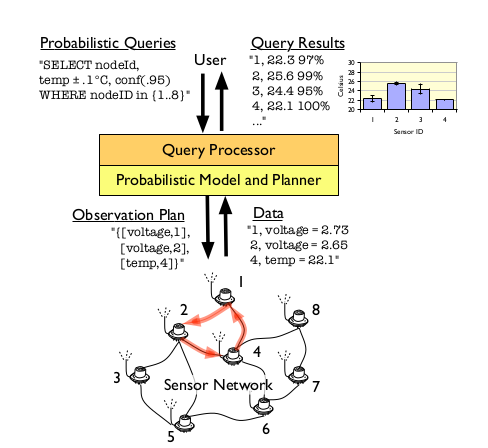
\includegraphics[width=\linewidth]{images/bbq-architecture.png}
\caption{Architecture of \textit{BBQ}~\cite{deshpande2004model}. A user writes
probabilistic queries in an \ac{SQL}-like language. The query processor plans
and executes the optimal query plan.}
\label{fig:bbq}
\centering
\end{figure}

The authors evaluated their system by comparing \textit{BBQ} with
TinyDB~\cite{madden2005tinydb} and Approximate-Caching on two datasets
collected by a small number of sensors (11 and 54 each). TinyDB is a sensor network
querying system in which the readings of sensor nodes are routed through the
network and aggregated on the way to the sink. With Approximate-Caching, sensor
nodes send their sensed values to a sink only if they differ from the previously
sent values by some user-defined margin $ \epsilon $. So in comparison, TinyDB
reports always the exact values asked for in a user query, while
Approximate-Caching is tweakable with error bounds, and \textit{BBQ} is
additionally configurable with \acp{CI}. Therefore, the acquisition costs of
TinyDB were constant while \textit{BBQ} outperformed the other algorithms on
high error margins ($ \epsilon = 1 $) with acquisition costs being an
order-of-magnitude lower than those of Approximate-Caching. As the authors
themselves point out, \textit{BBQ} is not suitable for anomaly detection, as
for such a task constant sensor sampling is required.

\par
\textit{9) Ken:}
Chu et al. tackle, i.a., this problem, in their work~\cite{chu2006approximate}.
The presented algorithm, \textit{Ken} targets \textit{SELECT *} queries in
which all values are requested from all sensor nodes. No data reduction takes
place, and such queries are thus expensive regarding energy consumption through
communication. \textit{Ken} operates using a prediction model which is
synchronized at the sink and sensor nodes. Users query the sensor network with
frequency and error interval arguments, e.g., values from all sensor nodes
every $ f $ seconds with an error margin of $ \pm\epsilon $. A sensor node
collects values and checks if the sink can predict the accumulated values
correctly within $ \pm\epsilon $. If the values lie within the interval, the
sensor node suppresses its reading. In the other case, the sensor node pushes
its values down the network to the sink. The models at the sink node use the
new values to \textit{resynchronize} its model with the model at the sensor
nodes. In a multihop \ac{SN}, additional compression based on spatial
correlation can take place at different hops. To enable compression based on
spatial correlation, the authors propose a clustering scheme in which there are
multiple clusters of sensor nodes with a cluster head each that communicates
with the sink. This reduces communication overhead, as sensor readings do not
have to be stored in one central place in the network. Each cluster head
maintains a synchronized prediction model with its child nodes. Additionally,
the sink maintains synchronized prediction models with the cluster heads. Such
a structure is depicted in Fig.~\ref{fig:cluster Chu}. To find such clustering
groups, the authors, i.a., present a heuristic approach, in which sensor nodes
are assigned to a cluster head by its data reduction factor, i.e., a
performance indicator for the prediction model. The cluster formation algorithm
is run at the sink, which induces some communication overhead if new clusters
have to be formed. The authors evaluated their approach on two real-world
datasets with small, fixed amount of sensors (one with 11 and the other with 49
sensors). \textit{Ken} was tested with the clustering technique and with an
average model, in which predictions are made with the average of all sensed
values, and no clusters are built. The authors came to a conclusion, that
\textit{Ken} performs better with the clustering scheme, when the communication
costs to the sink are many times higher than to a neighbor. This advantage
recedes if there are a lot of outliers which the model cannot predict.

\begin{figure}[h]
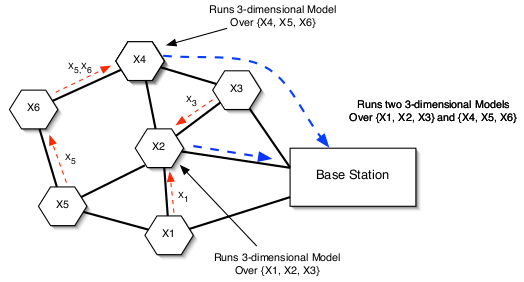
\includegraphics[width=\linewidth]{images/ken-clustering.png}
\caption{Example of a \ac{SN} with clusters by Chu et al.~\cite{chu2006approximate}}
\label{fig:cluster Chu}
\centering
\end{figure}

\par
\textit{10) ASAP:}
Gedik et al. point out in their work, that \textit{Ken} is ineffective when the
observed phenomenon changes unpredictably over time~\cite{gedik2007asap}. In
such cases, the prediction model has to be adapted or reconstructed, which
introduces high communication overhead if the model is constructed centrally at
the sink. Additionally, the authors of \textit{Ken} did not take the extra
energy expenditure of cluster heads have, compared to regular sensor nodes,
into account. Gedik et al. address these issues in their algorithm,
\textit{ASAP}. The algorithm organizes sensor nodes into clusters.
Clusterization is done periodically, i.e. every $ \tau_c $ seconds. This
enables rotation of cluster heads, preventing a premature power outage of a
sensor node. The formation of clusters and the selection of cluster heads is
done inside the network, without the mediation of the sink. Each sensor node
computes a probability of it becoming a cluster head, based on a user set
desired fraction of sensor nodes becoming cluster heads ($ f_c $) and the
sensor node's relative energy level to neighboring sensor nodes. Sensor nodes
which did not become cluster heads choose their cluster head by an attraction
factor, a combination of the hop distance to the cluster head and a weighted
data similarity with the readings of the cluster head and the sensor node, $
\alpha $. After clusters are constructed, cluster heads further division its
clusters into subclusters, of size $ \beta $, based on correlations between
each sensor node in the cluster. Initially, sensed values of \textit{all}
sensor nodes in a cluster have to be collected at the cluster head. This is
repeated every $ \tau_f $ seconds to update correlations and adapt to changing
dynamics in the observed phenomenon. The cluster head selects the fraction $
\sigma $ of sensor nodes to act as samplers in a subcluster, based on the
remaining energy of each sensor node. Only the sampler nodes and the cluster
head sense the environment (with a sampling rate of $ \tau_d $) and communicate
their sensed values to the sink. Additionally, cluster heads compute, for each
subcluster, a data mean vector and a covariance matrix which they send to the
sink as model parameters. The sink receives the sensed values from the sampler
nodes and predicts the values for the other sensor nodes.

Experiments were used to test messaging cost, network performance, energy
consumption and data quality. Centralized Exact and extreme variations of
\textit{ASAP} were used to compare the algorithm. The variations were a local
approach, in which predictions happens at the cluster heads and predicted
values are sent to the sink and a central approach in which all
predictions are carried out at the sink and values of all sensor nodes
for updating the model are also sent to the sink. The authors found
\textit{ASAP} outperforming the other algorithms in the number of messages sent
and the per sensor node energy consumption, while alternating, i.a., $ \sigma
$. The authors also studied the trade-off between the prediction error and
network lifetime, observing high lifetime improvements (90 \% longer lifetime in
comparison to centralized exact) if user-defined absolute error thresholds are
at around 1.

The authors point out that their algorithm is best suited for environmental
monitoring, as anomaly detection is not feasible due to only a subset of
sensors sensing at a time. Also, users should allow some prediction error to
utilize the algorithm effectively. The user can set all the parameters
described above, however, the authors suggest a configuration in their paper
which minimizes overhead.
\par

\textit{11) Jiang et al.:}
A similar paper by Jiang et al. was published in
2011~\cite{jiang2011prediction}. They make the point that the computational
overhead generated by prediction schemes may outweigh the energy savings
achieved by predicting a value at a sink rather than sending it through the
network. The algorithm utilizes clustering and duty cycling to increase energy
savings. Specifically, a sensor network is divided into clusters. Sensor nodes
which are not cluster heads, are either asleep or awake and sensing the
environment. Sensor nodes hold a history of predicted or sensed data points,
while cluster heads have a history of the values from all sensor nodes in their
cluster. Based on the historical data, an autoregressive model can be trained
to predict data locally at sensor nodes and cluster heads. Cluster heads issue
prediction bans to sensor nodes if a local prediction is less energy-efficient
than communicating the values to the cluster head, based on the predictability
of the data. The authors want to prevent sensor nodes computing a prediction if
the prediction is not accurate enough because the sensed data still has to be
sent. In such a case, the power used for the prediction is wasted. If no ban is
issued and the predicted value lies in the user-specified error bound, the
sensor node does not send anything and updates its local, historical data with
the predicted value. Else, the affected sensor node sends sampled data to the
cluster head and updates the local historical data with the sampled data. The
authors point out that in applications with data loss, acknowledgment messages
can be sent from sensor nodes to cluster heads, to counteract message failure.

The authors evaluated their approach on a synthetic dataset by varying the
ratio of transmission energy consumption and prediction energy consumption.
They compared their algorithm with and without the prediction ban feature and
concluded, that additional energy savings can be achieved when prediction cost
is high compared to communication cost. The authors point out that their
algorithm is not focussed on cluster creation. Algorithms like \textit{ASAP}
can be used to create clusters and cycle cluster heads.

\subsubsection{Adaptive Filtering}
\label{sec:Adaptive Filtering}

\textit{12) Jiang et al.:}
The first algorithm we would like to present in this category is a work from
2004 by Meng et al.~\cite{meng2004event}. Their approach focusses on in-network
spatial and temporal correlation based message suppression, based on Contour
Mapping. The authors describe Contour Mapping as a general technique in which
data points in a diagram are connected based on some similarities. Step size
can control the factor similarity. The authors use this technique to construct
Contour Maps in sensor networks so that not all sensor nodes with similar
readings have to send data. The suppression is done locally at every sensor,
while sinks interpolate suppressed readings of sensor nodes. For that, sensor
nodes sample their sensor every $ \tau $ seconds, while $ \tau $ is between $
\tau_{min} $ and $ \tau_{max} $. The sampling period is based on the magnitude
of the sensed value so an initial randomness factor is given. This is necessary
as some sensor nodes will report their readings first, while neighboring sensor
nodes listen for those readings. A sensor node which has overheard the values
of its neighbors, decides, based on the distance of its data to the average of
the neighbors' data $ \delta $ if it transmits its data. Additionally, a sensor
node may compare sampled values to $ m $ previous sampled values and based on
the same threshold $ \delta $ suppress or send its reading. Sensor nodes
consume some energy while overhearing messages sent by neighboring nodes. The
sinks know the geographical location of the sensor nodes and know which sensor
nodes (silent nodes) suppressed their readings. Thereby, the missing values of
the silent nodes can be interpolated by averaging the readings of nearby sensor
nodes. Additional smoothing can be done on the data by incorporating the values
of neighbors that are more than one hop away from a silent node as weighted
averages.

The authors tested, i.a., the accuracy and energy consumption of the approach
in a simulated environment, with 528 sensor nodes from which only 92 sent
readings to the sink in the course of the experiment. The maximum error did not
exceed 10, i.e., the distance between the value assigned to a silent node by
the sink and the actual value. With the introduction of network lossiness, 17
readings out of 92 are dropped on the way to the sink. In that case, the
maximum error was 20. Energy savings were compared against a centralized exact
scheme on transmitting data, listening for neighbors data and receiving data.
The algorithm achieved energy savings in each category of $ \approx88\% $ over
centralized exact.

% \begin{figure}
% \centering
% \begin{minipage}{.5\textwidth}
%   \centering
%   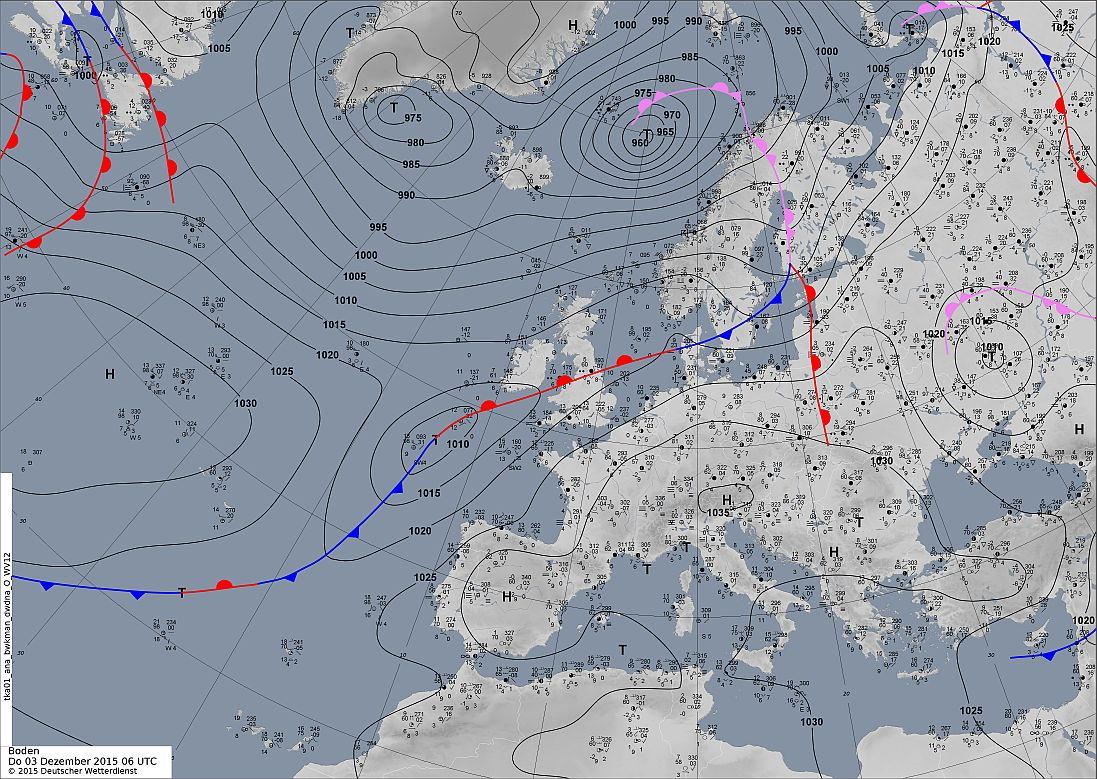
\includegraphics[width=\linewidth]{images/contour-map.jpg}
%   \captionof{figure}{Example of a contour map taken from the German Weather Agency (Deutscher Wetter Dienst)~\cite{dwd}}
%   \label{fig:contour map}
% \end{minipage}%
% \begin{minipage}{.5\textwidth}
%   \centering
%   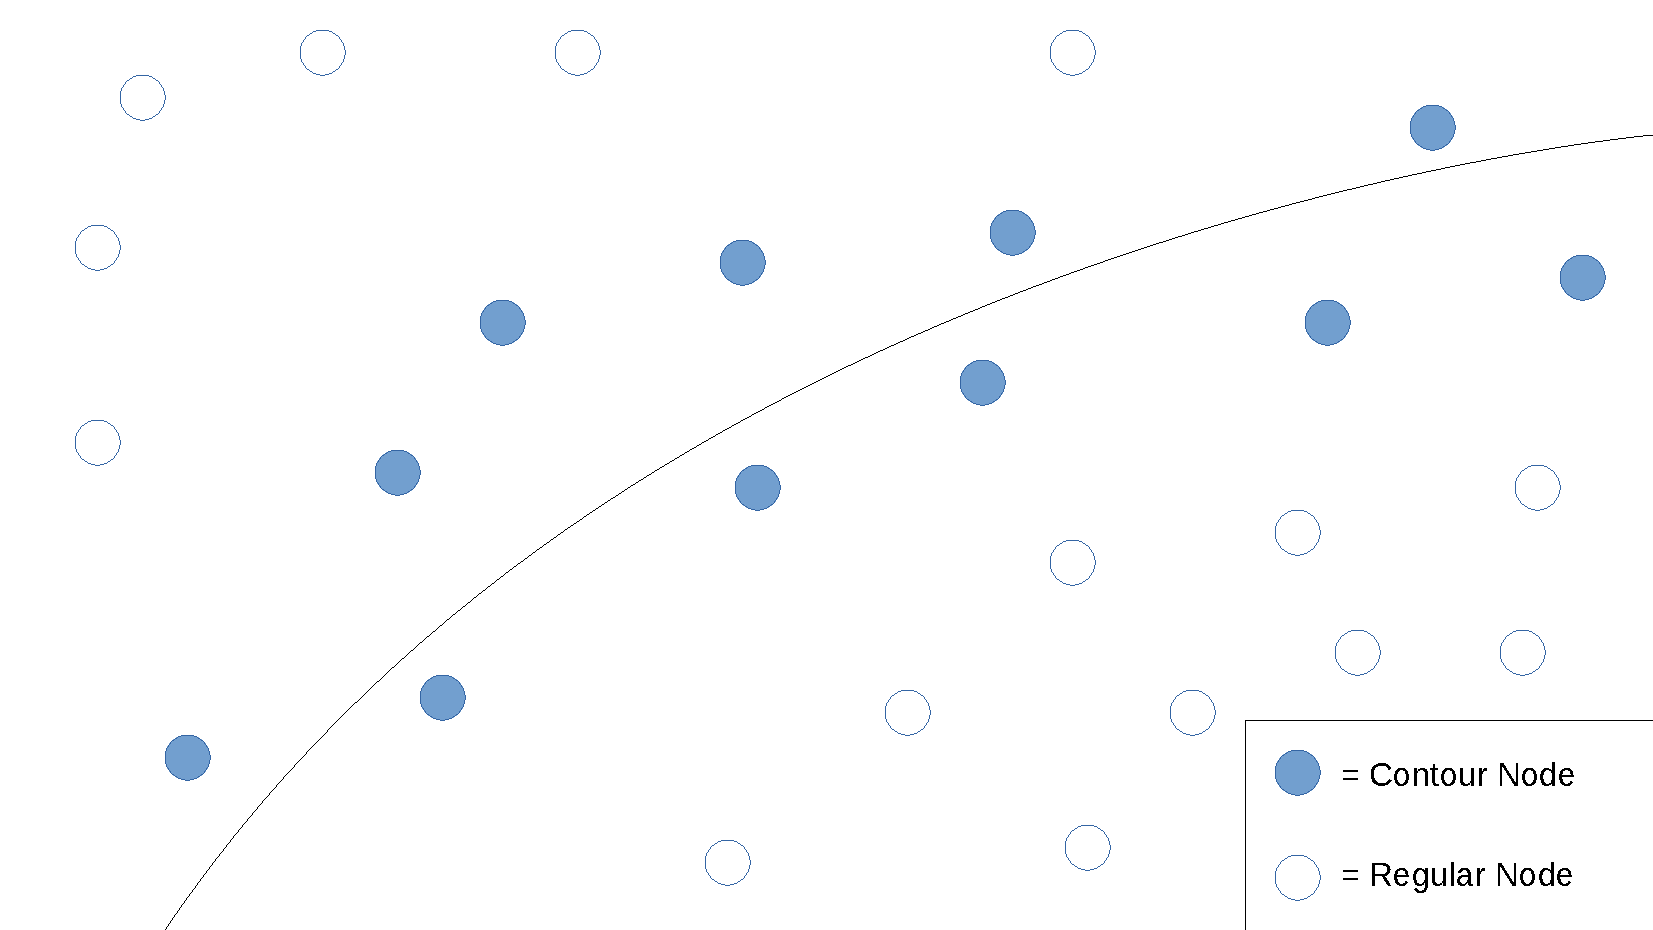
\includegraphics[width=\linewidth, height=5.3cm]{images/contour-nodes.pdf}
%   \captionof{figure}{Example of a contour line and contour (sensor) nodes~\cite{xu2008cme}}
%   \label{fig:contour nodes}
% \end{minipage}
% \end{figure}

\begin{figure}[h]
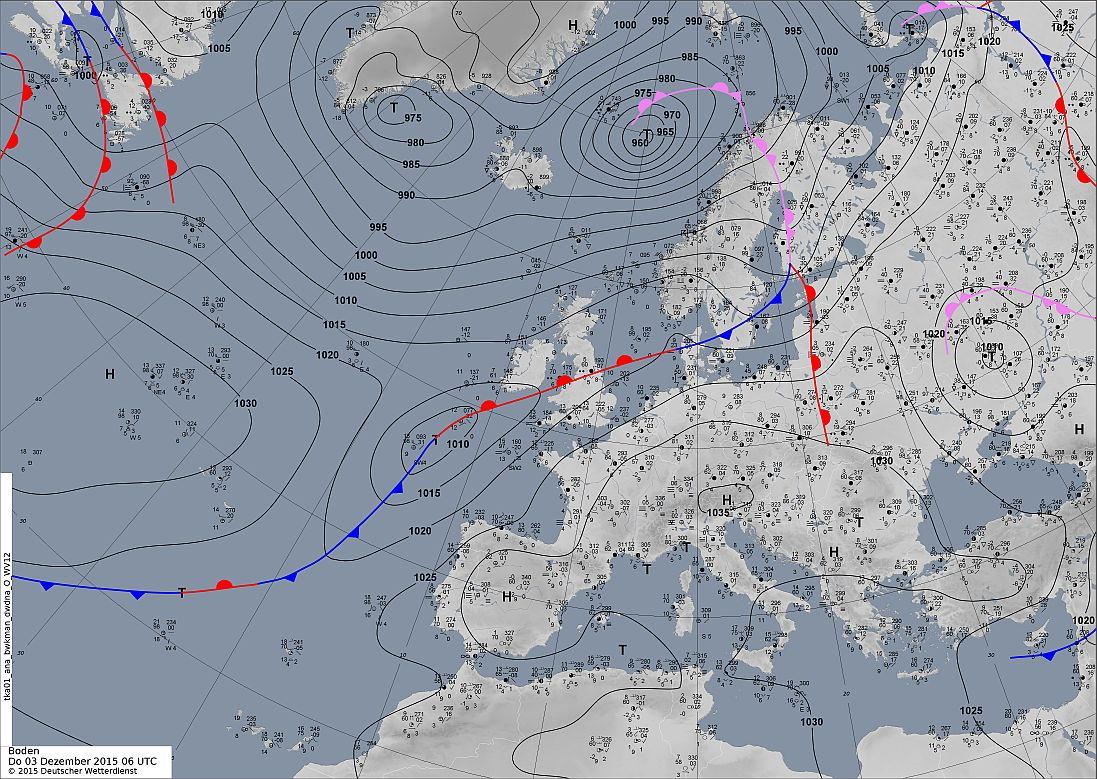
\includegraphics[width=\linewidth]{images/contour-map.jpg}
\caption{Example of a contour map taken from the German Weather Agency (Deutscher Wetter Dienst)~\cite{dwd}}
\label{fig:contour map}
\centering
\end{figure}

\textit{13) Solis et al.:}
Another algorithm, which leverages contour mapping to generate maps of
environmental phenomenons, is a paper by Solis et
al.~\cite{solis2005efficient}. Similar to the work of Meng et al., the
algorithm suppresses the reporting of readings at sensor nodes which are in the
same isocluster, i.e., there is no isoline between them. An example of isolines
in a contour map is given in Fig.~\ref{fig:contour map}. The space between
isolines is dependant on the application. Less space equals a higher data
resolution, as more potential isolines are between sensor nodes, at the expense
of energy, as more readings are communicated. The area between isolines is user
configured and propagated to all sensor nodes. An isoline can move if a sensor
node senses a reading which differs from a previous reading by the user set
space. The sensor node broadcasts the change in isolines to its neighbors.
Readings are scheduled from the farthest leaf nodes (in the case of a tree
topology) to the sink. This enables additional energy conservation, as sensor
nodes go into a sleep mode after sampling their sensors. The authors indicate
that further temporal suppression is applicable, as sensor nodes may only
report a reading if that reading changed the isocluster. The authors evaluated
their approach in a simulated environment against multiple other approaches,
e.g., an aggregation scheme, in which data is aggregated at parent nodes into
groups, and the averages of the groups are sent further down the network. The
other schemes were a centralized exact approach with and without additional
temporal suppression. The authors found their approach outperforming the other
algorithms in energy savings and accuracy when constructing contour maps from
sensor readings.

\textit{14) Conch:}
A paper by Silberstein et al.~\cite{silberstein2006constraint} presents a
technique, \textit{Conch}, with which redundant reporting can be reduced even
further compared to the two previous presented schemes. The authors argue that
both algorithms do not leverage the relative differences of sensor nodes
values, i.e., when two sensor nodes differ significantly in their readings, but
one reading can always be inferred from the other one, and no values should be
sent. In \textit{Conch} a sensor node in a network has a set of sensor nodes
from which it receives updates (updaters) and a set of sensor nodes to which it
sends updates to (reporters). A sensor node broadcasts its sensed values to the
reporters if its new sensed value differs from the old sensed value by some
margin. When a sensor node receives a value from an updater node, it computes
the difference to its own sensed value. If no value is received, the sensor
node assumes no change has taken place. The sink monitors all differences
between sensor nodes (called edges by the authors), so in the initialization,
all reporters send their edges to the sink. Some sensor nodes are monitored
directly. The directly monitored sensor nodes route their sensed values and
their edges to the sink directly. At every time step, which derives from a user
set sampling frequency, the sink receives updated edges from reporting nodes
and sensed values from directly monitored sensor nodes. This enables the sink
to compute the value of every sensor node at any time step if every sensor node
can be reached from a directly monitored sensor node and the corresponding
edges. The authors emphasize that \textit{Conch} is a monitoring algorithm;
routing schemes are still used to route a report from a sensor node to the sink
efficiently. The algorithm is flexible as the authors present ways to build
\textit{Conch plans}, i.e., monitoring topologies, to focus on minimizing
energy consumption or increase sensor node and message failure resilience. The
authors tested their algorithm in different simulated environments against
multiple algorithms, i.a. the scheme by Meng et al.~\cite{meng2004event}. The
authors tested the performance of \textit{Conch} on, i.a. \acp{SN} with
different sensor node densities, predictable increases of the observed value
and outlier detection. \textit{Conch} outperforms all other schemes in terms of
energy consumption at every test and only the scheme of Meng et al. exhibits
similar energy consumption levels with increasing sensor density.

\textit{15) \ac{CME}}: A paper from Xu et al.~\cite{xu2008cme} presents another
contour mapping approach, utilizing binary classification and clustering to
detect contours and reduce the total number of transmitting sensor nodes.
Different from the scheme of Solis et al., the authors employ clustering to
contour maps. The authors define a contour as "a curve that connects points
with equal feature values." The range between two contours is application
specific. The authors use the term contour \textit{node} to describe sensor
nodes which have a reading that belongs to a different contour range than a
neighboring sensor nodes' reading. All nodes participate in contour node
identification in a cluster by broadcasting their sampled values. An example of
a contour and contour nodes is given in Fig.~\ref{fig:contour nodes}. Only
contour nodes communicate their readings to the cluster head. The authors
employ \ac{SVM} at the cluster head to classify sensor nodes' membership to one
side of the contour. The cluster head can compute the contour segment of its
cluster which it then sends to the sink. At the sink, the contour map of the
network can be constructed. The authors point out that in a multi-hop routing
scheme additional aggregation can take place at routing cluster heads.

The authors evaluated their approach in a simulated event detection scenario
with 2500 sensor nodes. The authors compared their algorithm against multiple
other schemes, i.a. a centralized exact and the scheme of Solis et
al.~\cite{solis2005efficient} which they dubbed "isolines". The authors tested
the algorithms on energy consumption and contour map accuracy while varying
different contour step and network sizes. \ac{CME} outperformed every algorithm
in every test. The isoline approach exhibited similar accuracy under
increased energy expenditure.

\begin{figure}[h]
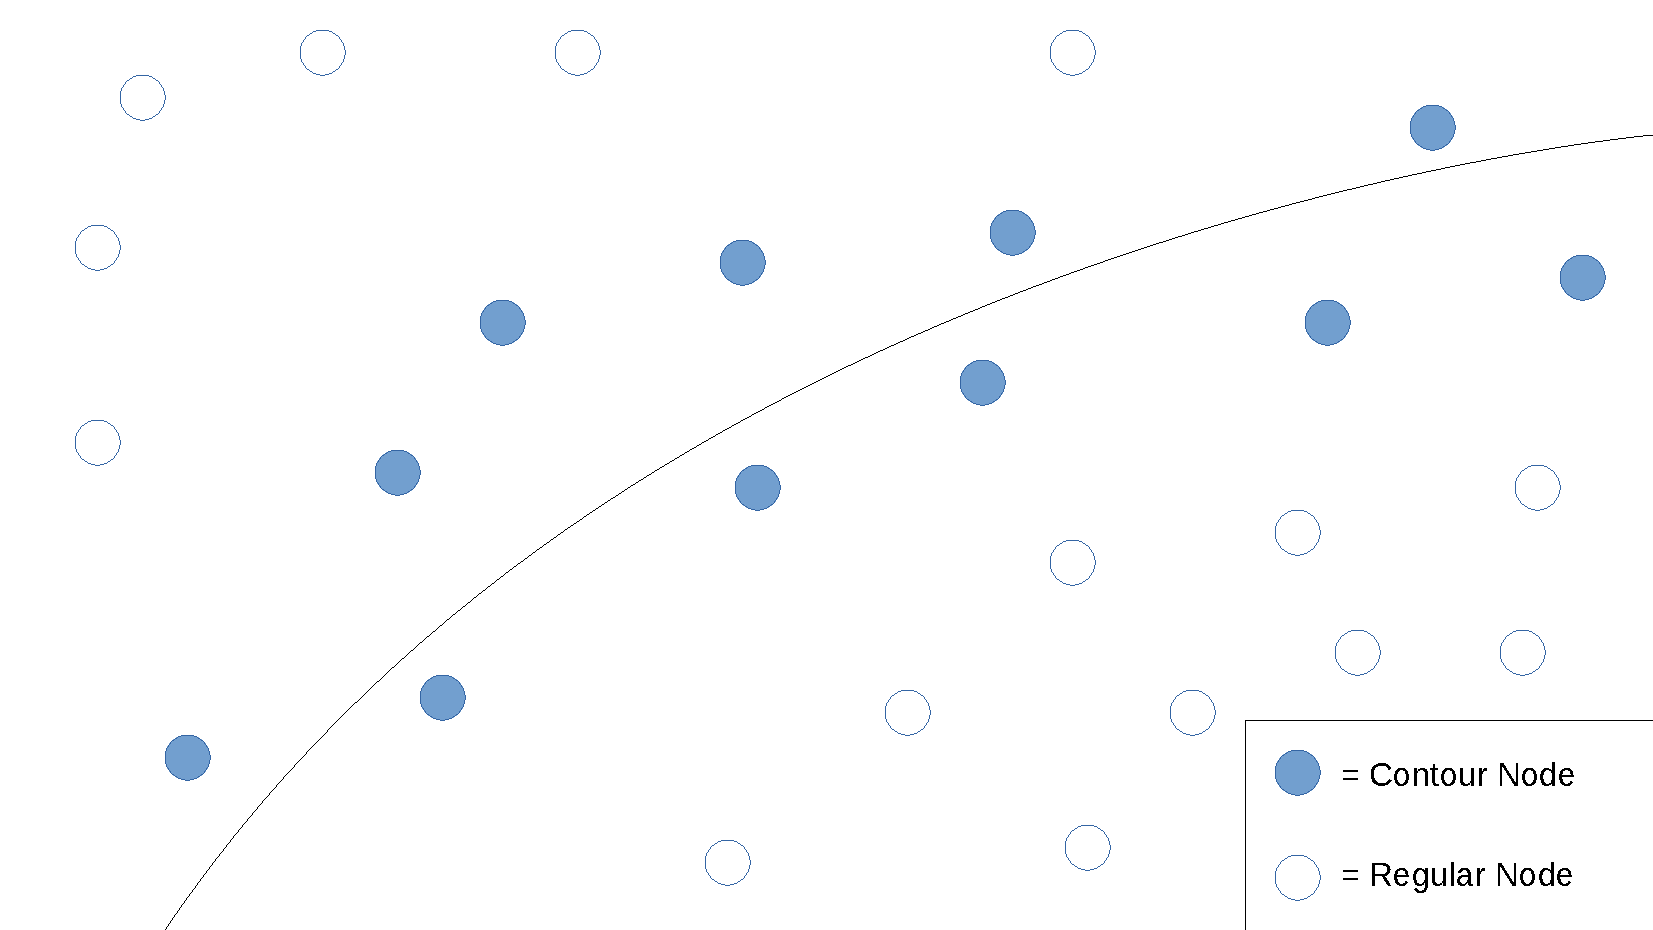
\includegraphics[width=\linewidth]{images/contour-nodes.pdf}
\caption{Example of a contour line and contour (sensor) nodes~\cite{xu2008cme}}
\label{fig:contour nodes}
\centering
\end{figure}

\FloatBarrier

\section{Related Algorithms}
\label{sec:Related Algorithms}

In this section, we will present additional algorithms from the area of
routing~\ref{sec:Routing} and topology control~\ref{sec:Topology Control}. We
will also present possible combinations of algorithms which could inspire
further research in the area of data sampling from sensor networks
~\ref{sec:Combination of Algorithms}.

We decided to include routing and topology control as additional classes of
algorithms in \acp{SN}, because  all of the schemes described in the taxonomy
use (e.g.~\cite{padhy2006utility}) or presume
(e.g.~\cite{silberstein2006constraint}) some routing and topology control
scheme. Multiple exhaustive surveys on topology control~\cite{aziz2013survey,
li2013survey} and routing~\cite{al2004routing, pantazis2013energy,
singh2010routing} exist already. We will nevertheless show some examples of
routing and topology control algorithms, as this will grant a better overview
of the challenges of data sampling in \acp{SN}.

\subsection{Routing Schemes}
\label{sec:Routing}

Routing schemes define how data is communicated in a network. In a survey from
2004 on routing protocols, Al-Karaki et al.~\cite{al2004routing} classify
routing into network protocols and routing criteria. Network protocols define,
how communication between sensor nodes in a sensor network is structured. With
flat network routing, all sensor nodes have the same task in the network,
mainly sensing and forwarding data. Hierarchical network routing incorporates
schemes, in which the sensor network is divided into clusters. We presented
such a scheme in our taxonomy with \textit{ASAP}~\cite{gedik2007asap}. In
location-based routing, sensor nodes are typically equipped with a GPS
module~\cite{xu2001geography} or can infer their position on based on the
strength of incoming signals, if a GPS module is too
expensive~\cite{hu2004localization}. Location-based routing is especially
useful in mobile sensor networks, in which sensor nodes change their position
in the sensing field frequently and therefore change their
neighbors~\cite{hu2004localization}.

A work by Zou et al.~\cite{zou2004pager} introduces a \textit{stateless},
(sensor nodes do not have to save past routing paths) location-based routing
algorithm, \textit{PAGER-M}, for mobile sensor networks. The algorithm uses
greedy forwarding~\cite{stojmenovic2001loop} to rout sensed data to the next
sensor node on the shortest path to the sink. However, sensor nodes can
sometimes be the closest sensor node to the sink in their local topology (but
still out of range to transmit), even though there exists a shorter path and
thus routing can fail, e.g., Fig.~\ref{fig:shadow nodes}. To handle such cases,
the authors define a scheme which identifies such sensor nodes. Sensor nodes
assign cost variables to themselves, based on the cost variables of its
neighbors. This ensures that every sensor node has a neighbor with a lower cost
variable than itself, which enables a high-cost-to-low-cost routing if greedy
routing fails. The authors tested their algorithm against
\textit{GPSR}~\cite{karp2000gpsr} and \textit{AODV}~\cite{perkins2003ad} in a
simulated environment with ns-2. \textit{GPSR} is a stateless routing algorithm
which uses greedy routing and perimeter routing when greedy routing fails.
Perimeter routing uses the right-hand rule to traverse a graph
counter-clockwise. AODV is a routing algorithm in which sensor nodes maintain
routing paths to frequently communicated sensor nodes. If no path is known
pathfinding is initiated by broadcasting a route request message.
\textit{PAGER-M} outperformed the other algorithms in package delivery ratio,
as the algorithm uses a conservative path choosing, i.e., a longer routing path
is chosen if a sensor node on the shorter path is moving aways thus increasing
package loss probability. \textit{GPSR} found the shortest paths on average in
the experiment, when sensor nodes had lower communication ranges. However, the
routing overhead and energy consumption were consistently higher with
\textit{GPSR} compared to \textit{PAGER-M}.

\begin{figure}[h]
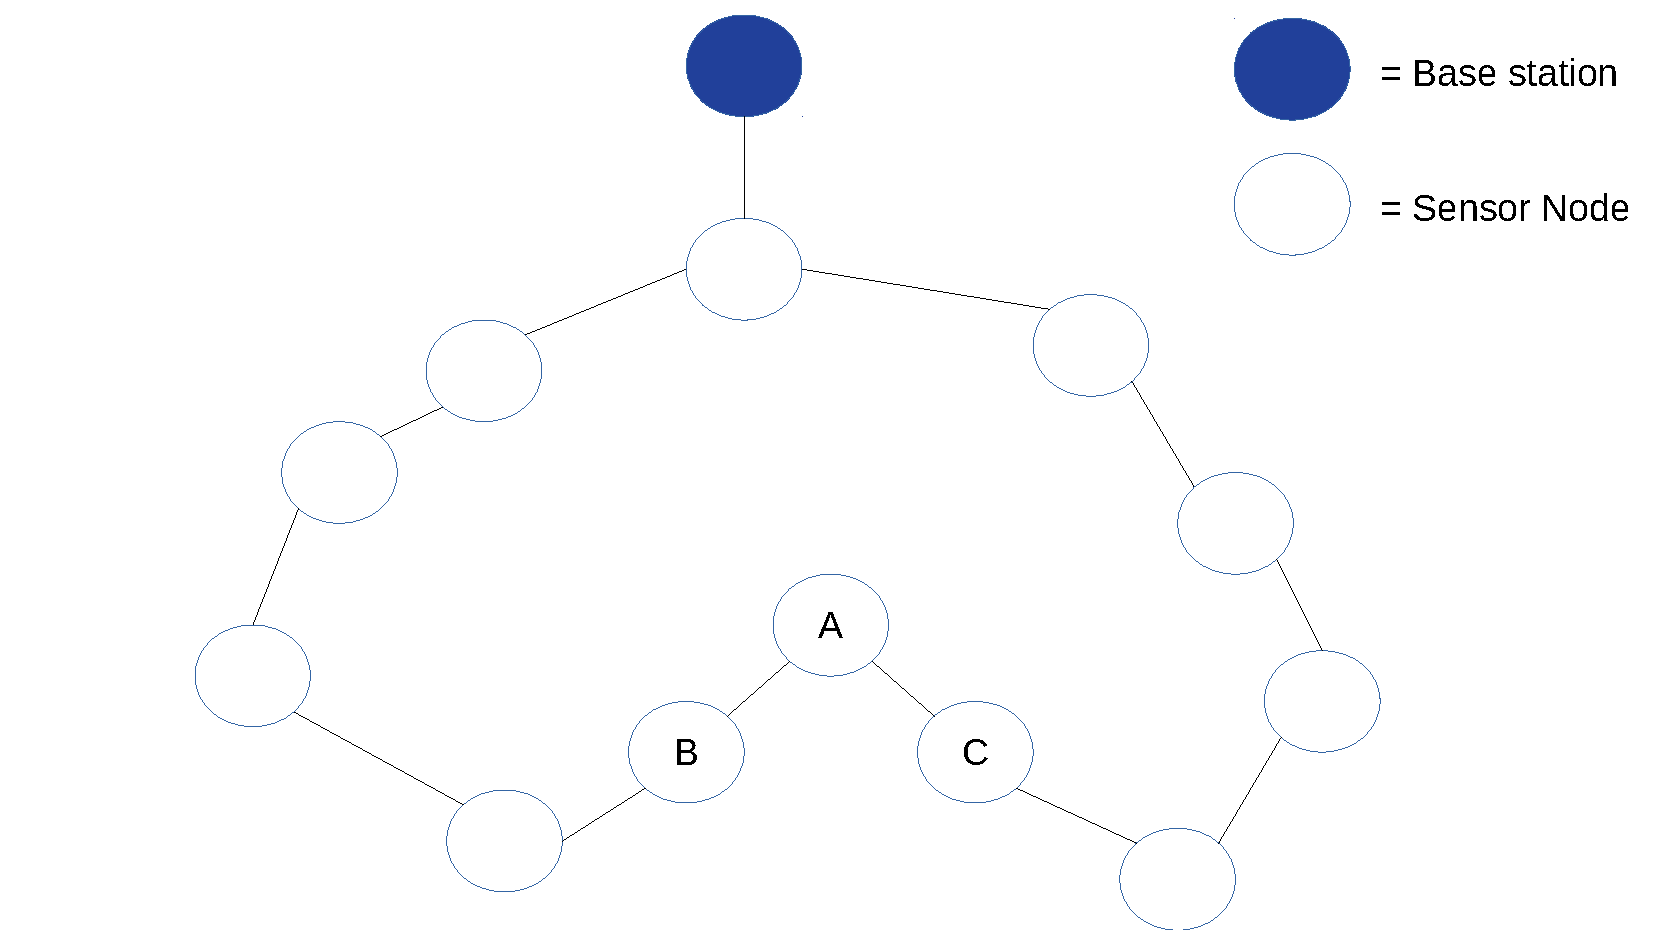
\includegraphics[width=\linewidth]{images/pager-shadow-nodes.pdf}
\caption{Example of a topology where greedy routing can fail. Sensor node A is
the closest sensor node to the sink in its local topology~\cite{zou2004pager}.}
\label{fig:shadow nodes}
\centering
\end{figure}

Pantazis et al. extend the work of Al-Karaki et al. in their survey on routing
protocols~\cite{pantazis2013energy}, with, i.a., Mobile Agent-based protocols.
Such protocols use mobile agents, i.e., software, to visit sensor nodes and
perform tasks, therefore making the \ac{SN} more flexible. Chen et
al.~\cite{chen2007applications}, i.a. justify Mobile Agent-based protocols as a
means to run multiple applications on the same \ac{SN}. As it is unfeasible to
store all application specific programs at each sensor node (due to resource
constraints), mobile agents can be used to migrate between sensor nodes and
perform application specific tasks autonomously.

Chen et al. present multiple algorithms for mobile agent-based protocols in
their work~\cite{chen2011itinerary}. The authors expand with their algorithms
the \textit{LCF} algorithm by Qi et al.~\cite{qi2001optimal}. \textit{LCF}
calculates an ad-hoc itinerary (application specified route through sensor
nodes) by searching for the closest sensor node to a current sensor node. Chen
et al. expand the algorithm by presenting a scheme to select the first sensor
node in the itinerary which would minimize the energy expenditure of the mobile
agent. The authors further propose an algorithm to iteratively optimize the
next $ k $ hops of the mobile agent. The authors find in their experiments, in
which they simulate a large-scale \ac{SN} with 800 sensor nodes, that their
algorithm decreases the energy-delay product ($ energy \cdot delay $) by 80\%
in the first iteration and only marginally in following iterations.

Singh et al.~\cite{singh2010routing} additionally define single-path and
multi-path routing. With single-path routing, sensor nodes send their sensed
values on the shortest path to the sink. With multi-path routing, on the other
hand, sensor nodes divide their sensed data and send it with the \textit{k}
shortest routes to the sink. The authors additionally define different
instances of multi-path routing, e.g., disjoint paths and braided paths. With
disjoint paths, each path has different sensor nodes, while in braided paths a
primary path is built and additional paths are computed by excluding one sensor
node from the primary path.

Chen et al.~\cite{chen2011itinerary} present an algorithm, \ac{DGR}, for
routing real-time video data over multiple paths in a \ac{WSN}. \acp{WSN} which
transmit highly compressed video streams are also called \acp{VSN}. In
\acp{VSN} only a few sensor nodes are equipped with video capturing divides and
more powerful batteries. The rest of the nodes are do not have such equipment
and only serve as relay nodes. The authors argue that \acp{VSN} are limited in
bandwidth and energy and are additionally susceptible to transmission errors.
The algorithm constructs an application specific number of \textit{disjoint}
paths from a source video sensor node to the sink. To keep the paths disjoint,
the algorithm may construct routes which have nodes that are further away from
the sink than the source node. Such cases can occur when the node density is
low in the \ac{SN}, and the path number is high. The authors argue that
disjoint paths are important, as video sent on intersecting paths "interferes
with each other severely". Next hop selection is made in the algorithm by
broadcasting probe messages from the source to the next hop and so on. A node
is selected a the next hop based on its location, i.e., distance to the
\textit{StrategicMappingLocation}, which is a point on the line between the
source node and the sink. The authors tested their algorithm in a simulated
environment with 500 sensor nodes, one video sensor node and one sink against
the already covered \textit{GPSR} with and without additional \ac{FEC}
\footnote{The authors define \ac{FEC} as a scheme which is used to increase
error resilience in real-time video transmission by generating redundant
packets.} coding. The authors' simulations show that their scheme outperforms
\textit{GPSR} with and without \ac{FEC} coding in terms of $ \eta $. The metric
$ \eta $ is defined by the authors as $ \eta = \frac{lifetime \cdot
PSNR}{delay}$ with $ lifetime $ specifying the time until the first sensor
nodes dies, $ PSNR $ as peak signal-to-noise ration, i.e., the received video
quality, and $ delay $ denoting the "average delay for real-time video
applications."

\subsection{Topology Control}
\label{sec:Topology Control}

Aziz et al. define topology Control.~\cite{aziz2013survey} as "a technique that
uses any controlled network parameter to generate and maintain a topology for
the benefits of reducing energy consumption and achieving the desired property
for an entire network." The authors list modifiable parameters as the
transmission power of the radio, changing the mode of sensor nodes, and
clustering. Sensor nodes can manipulate the transmission power of their
transceivers to vary the transmission range and therefore reduce energy
expenditure for communication. While clustering is also mentioned as a
\textit{routing} technique, changing modes of sensor nodes is a new
classification, also called \textit{duty cycling}~\cite{carrano2014survey,
lin2004medium, buettner2006x}. As Carrano et al. point
out~\cite{carrano2014survey}, duty cycling finds a tradeoff between latency and
energy consumption in \acp{SN}. End-to-end latency increases, if routing sensor
nodes have to wait for the next sensor node in the routing path to wake up.
Additionally, the authors argue, that although a sensor node consumes less
energy in sleep mode, i.e., the radio transceiver is turned off, higher data
collision rates and potential control packet overhead, induced by duty cycling,
can increase energy expenditure.

Sun et al.~\cite{sun2008ri} present a \ac{MAC} protocol which tackles the
problems mentioned above. With the protocol \textit{RI-MAC} every sensor node
has a wake-up schedule. While awake, a sensor node will broadcast a message
that it is ready to receive data. A sender node, which is awake and waiting for
the message, then starts data transmission, which the receiving sensor node
acknowledges. The authors argue, that due to the receiver initiated
transmission, \textit{RI-MAC} handles heavier traffic loads more power
efficient than other \ac{MAC} protocols, such as \textit{B-MAC} and
\textit{X-MAC}. This is because the broadcasted message by a receiver sensor
node has a backoff window size with which the receiver can schedule different
sender nodes. The authors tested their protocol extensively on a small,
real-world testbed and in a large \ac{SN} simulated with the ns-2
tool~\cite{bajaj1999improving}. Their tests were additionally run on
\textit{X-MAC}~\cite{buettner2006x}, in which the receiver does not initiate
data transmission, and \textit{X-MAC-UMPA} which is a simplification of
\textit{X-MAC}. In both test environments, \textit{RI-MAC} outperformed the
other two algorithms in, i.a. average packet delivery ratio and average
latency.

Li et al.~\cite{li2013survey} address in their survey on topology control,
network coverage as a vital issue in \acp{SN}. The authors define network
coverage as "the surveillance map of the target field, which emphasizes the
sensors' placement positions and cooperations among sensors." A target field
has observable points and can be covered by sensor nodes to monitor every point
in the field. The authors define such coverage as blanket coverage. Barrier
coverage is a type of topology where the sensor nodes are laid out in such a
way, that the outlines of a field are monitored. Liu et
al.~\cite{liu2008strong} define a barrier as "the union of the covered areas of
sensors." Barrier coverage can be used to spot intruders if they cross an area
covered by a sensor node. However, barrier coverages can have gaps (e.g.
Fig.~\ref{fig:coverage}), especially if the sensor nodes are deployed randomly,
e.g., dropped from an airplane, and have scheduling mechanisms to turn off
their sensors~\cite{liu2008strong}. The algorithm divides the observed area
into smaller regions. Each region is divided into disjoint segments, where
sensor nodes are distributed horizontally, and vertical strip, where sensor
nodes are distributed vertically. Afterward, the algorithm computes how many
disjoint segments need to be active to provide full barrier coverage with no
gaps. Through rotation of the active segments, a more extended network lifetime
can be achieved. The authors tested their approach in a simulated environment
against a centralized approach, i.e., barriers are computed for the whole area.
The authors found that their algorithm forms stronger barriers, i.e., more
local barriers are found in the segments than across the entire area.
Additionally, the authors argue that their algorithm has lower communication
overhead and computational costs than the centralized algorithm because sensor
nodes only have to communicate in their local segments.

% TODO Potentially add 3D sensor networks and Sweep Coverage

\begin{figure}
\begin{subfigure}{.5\textwidth}
  \centering
  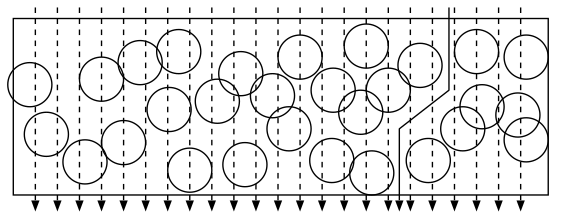
\includegraphics[width=.8\linewidth]{images/weak-coverage.png}
  \caption{}
  \label{fig:weak}
\end{subfigure}%
\begin{subfigure}{.5\textwidth}
  \centering
  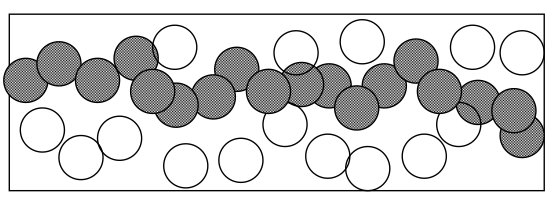
\includegraphics[width=.8\linewidth]{images/strong-coverage.png}
  \caption{}
  \label{fig:strong}
\end{subfigure}
\caption{Example of a weak (a) and a strong (b) barrier coverage \ac{SN}}
\label{fig:coverage}
\end{figure}

\FloatBarrier

\subsection{Combination of Algorithms}
\label{sec:Combination of Algorithms}

In this section, we will present possible combinations of algorithms showcased
in this thesis. Additionally, we will present schemes, which employ multiple
techniques categorized by us as different classes. As most of the algorithms
filed focus only on a specific area of data gathering in sensor networks, they
are not able to function without a routing scheme or topology control. For
example, Srbinovski et al.~\cite{srbinovski2016energy} focus entirely on their
adaptive sampling algorithm, while Padhy et al.~\cite{padhy2006utility} present
a routing scheme \textit{and} an adaptive sampling scheme. To utilize the
algorithm of Srbinovski et al. in a \ac{SN}, a routing technique and topology
control schemes are needed. We will not discuss such combinations as they are
application specific and would go beyond the scope of this thesis.

Trihinas et al.~\cite{trihinas2015adam} present \textit{AdAM}, a framework
which incorporates a sampling \textit{and} a filtering algorithm. With
\textit{AdAM} running on sensor nodes, a data stream $ M $ is estimated to
reduce the number of sampling periods when the metric stream does not fluctuate
and vice versa. A sampling period $ T_i $ is computed by estimating the metric
stream evolution. The authors use a \ac{PEWMA} to produce an estimated metric
stream $ M' $. The \ac{PEWMA} is a Variation of \ac{EWMA} which provides a
one-step-ahead estimation. The authors state that \ac{PEWMA} is more robust
against abrupt transient changes in the metric evolution than \ac{EWMA}. When $
M' $ differs from $ M $ by a user-specified imprecision value $
\gamma $, then $ T_i $ is increased to a maximum sampling period $ T_{max}
$. Otherwise $ T_i $ is decreased to a minimal sampling period $ T_{min} $.
Additionally, sampled data points $ v_{i} $ can be temporally suppressed if
they lie in a user-specified interval $ v_i \in [v_{i-1} - R_i, v_{i-1} + R_i]
$ where $ R_i $ is the adaptable filter range. With \textit{AdAM}, an adaptive
filtering range is computed at a sensor node at every time step $ i $. The Fano
Factor is utilized to measure the variability of the data stream at the current
timestep, i.e., if the variance of the data stream rises, then so does the Fano
Factor. The Fano Factor is then compared against $ \gamma $. $ R_{i+1} $ is
shortened if the Fano Factor is greater than $ \gamma $ and widened if the Fano
Factor is less than $ \gamma $.

Chatterjea et al.~\cite{chatterjea2008adaptive} present in their work an
approach, which leverages model-based prediction and adaptive sampling to
reduce energy expenditure in \acp{WSN} with energy-hungry sensors. First, a
buffer $ r $ with a user-specified length is filled at every sensor node with
sampled values at a user-specified sampling period. Afterward, at each
consecutive period, a sample is taken, and an amount is predicted with a time
series model (the authors use a \ac{ARMA} model). If the prediction falls
within a user-specified error margin, $ \delta $, a counter \textit{CSSL} is
incremented by 1, specifying the number of next sampling periods to skip. The
maximum value the counter can take is based on how many neighbors, which also
can detect an event, a sensor node has. Correct predictions are stored in the
buffer, and if predictions do not satisfy the error margin, sampled values are
stored at the buffer and \textit{CSSL} is reset to 0. Additionally, the sink
stores the prediction models of every sensor node. Initially, all sensor nodes
send their model parameters to the sink and keep a copy of the send model
locally. If a sensor node detects an inaccurate prediction at the sink, it
sends an updated sink model to the sink. The authors point out that their
algorithm is not suitable for time-critical applications, as it detects events
at a high probability, but not as soon as they occur.

The essence of the two works presented is that multiple techniques can be used
to reduce sampling in periods of low variability of an observed signal and
further reduce communication loads by suppressing the already sampled values or
predicting them at a sink. The authors of
\textit{Backcasting}~\cite{willett2004backcasting} criticize their algorithm,
as it lacks a cluster head rotation scheme. As cluster heads generally
coordinate the sensing tasks of sensor nodes in their cluster, they consume
more energy than normal sensor nodes~\cite{pradhan2016cluster}. Additionally,
ad hoc cluster formation and thus cluster head cycling is important in
countering general node failure~\cite{hu2018fault}. A possible addition to
\textit{Backcasting} could be the clustering algorithm presented in
\textit{ASAP}~\cite{gedik2007asap}. As the \textit{Backcasting} algorithm
activates clusters to perform sensing tasks, \textit{ASAP} could be used to
select cluster heads in a cluster periodically, to spread the energy load.

Another possible combination could be the \textit{ASAP} algorithm and another
adaptive sampling algorithm. For example, the \ac{USAC} algorithm could be used
to dynamically adapt the sampling rate of a sensor node based on the dynamics
of the observed phenomenon. Additionally, the model, which runs at sensor
nodes, could be shifted to run at a cluster head. The model could then also run
on the sink. Similar to the scheme of Chatterjea et
al.~\cite{chatterjea2008adaptive}, only the model parameters would be sent to
the sink, if the cluster head detects an incorrect prediction. The difference
to the scheme of Chatterjea et al. is the additional clustering of the sensor
nodes. 

The authors of the \textit{Conch} algorithm point
out~\cite{silberstein2006constraint}, that their scheme can be used in
combination with a prediction scheme like \textit{Ken}~\cite{jain2004adaptive}.
Similar to \textit{ASAP}, \textit{Ken} could predict values of cluster members
at cluster heads and route values to the sink if the prediction is not accurate
enough. The \textit{Conch} scheme could then be used in a multi-hop sensor
network to additionally suppress values which are routed through the
intermediary routing nodes.

\section{Conclusion}

With the increase of network-connected devices~\cite{gartner} that produce huge
amounts of data at high velocities, we need efficient sampling algorithms to
extract the most important information from the data without processing all of
it. To enable large-scale sensor networks, data sampling and data reduction
have to happen at or near the sensors. Our focus in this thesis lies on sensor
networks. However, we argue that the presented algorithms and challenges apply
to all kinds of distributed systems. We presented in this thesis a catalog of
sampling algorithms for sensor data. We showcased algorithms from the areas of
\textit{adaptive sampling}, \textit{compressive sampling}, \textit{model based
schemes}, and \textit{adaptive filtering}. We summarized our findings in a
taxonomy and summed up the evaluation of the algorithms in a table. We
additionally presented algorithms from other areas than sampling and filtering,
i.e., \textit{routing} and \textit{topology control}, to create a complete
picture of the challenges in data gathering in \acp{SN}. We additionally showed
possible combinations of algorithms presented in this thesis.